% Document class and language
\documentclass{article}
\usepackage{polski}
\usepackage{hyperref}
\usepackage{biblatex}

\addbibresource{literatura.bib}
% Setting geometry
\usepackage[a4paper,top=2cm,bottom=2cm,left=3cm,right=3cm,marginparwidth=1.75cm]{geometry}

% Useful packages
\usepackage{csvsimple}
\usepackage{graphicx}
\usepackage{subcaption}
\usepackage{forest}
\usepackage{listings}
\usepackage{indentfirst}
\lstset{language=Python}

\usepackage{xcolor}

\definecolor{codegreen}{rgb}{0,0.6,0}
\definecolor{codegray}{rgb}{0.5,0.5,0.5}
\definecolor{codepurple}{rgb}{0.58,0,0.82}
\definecolor{backcolour}{rgb}{0.95,0.95,0.92}

\lstdefinestyle{pythonstyle}{
    backgroundcolor=\color{backcolour},   
    commentstyle=\color{codegreen},
    keywordstyle=\color{magenta},
    numberstyle=\tiny\color{codegray},
    stringstyle=\color{codepurple},
    basicstyle=\ttfamily\footnotesize,
    breakatwhitespace=false,         
    breaklines=true,                 
    captionpos=b,                    
    keepspaces=true,                 
    numbers=left,                    
    numbersep=5pt,                  
    showspaces=false,                
    showstringspaces=false,
    showtabs=false,                  
    tabsize=2
}

\lstdefinestyle{basicstyle}{
    backgroundcolor=\color{backcolour},   
    basicstyle=\ttfamily\footnotesize,
    breakatwhitespace=false,         
    breaklines=true,                 
    captionpos=b,                    
    keepspaces=true,                 
    numbers=left,                    
    numbersep=5pt,                  
    showspaces=false,                
    showstringspaces=false,
    showtabs=false,                  
    tabsize=2
}

\lstset{style=pythonstyle}

\setcounter{secnumdepth}{3}


\title{Metoda trójwymiarowego modelowania obszarów urbanistycznych z wykorzystaniem metod fotogrametrii}

\author{
    \small Daniel Borkowski\\
    \and
    \small Julia Farganus\\
    \and
    \small Rafał Mielniczuk\\
    \and
    \small Katarzyna Wochal\\
}
\date{12.2024}
\renewcommand\refname{Źródła}

\begin{document}


\begin{titlepage}
    \begin{center}
        \Large
        Politechnika Wrocławska\\
        Wydział Informatyki i Telekomunikacji\\
        \vspace*{1cm}
            
        \Huge
        \textbf{ZESPOŁOWE PRZEDSIĘWZIĘCIE INŻYNIERSKIE}

        \vspace{1.5cm}
        \huge
        \textbf{Metoda trójwymiarowego modelowania obszarów urbanistycznych \\z wykorzystaniem metod fotogrametrii}

        \vspace{1.5cm}
        \LARGE
        Daniel Borkowski\\
        Julia Farganus\\
        Rafał Mielniczuk\\
        Katarzyna Wochal\\

        \vspace{1.5cm}
        Opiekun pracy\\
        dr hab. inż. Marek Krótkiewicz, prof. PWr

        \vfill
            
            
        \vspace{0.8cm}
            
            
        \Large
        Wrocław, 2024
        
            
    \end{center}
\end{titlepage}

\tableofcontents

\section{Wprowadzenie}

Przedmiotem projektu było wykonanie aplikacji wykorzystującej metody fotogrametrii do modelowania trójwymiarowych scen miejskich. Zaimplementowany program umożliwia użytkownikowi zrekonstruowanie chmury punktów i modelu 3D na podstawie podanych na wejściu zdjęć fotogrametrycznych za pomocą dostosowanych do specyfiki problemu w toku eksperymentów rozwiązań \textit{structure from motion} i \textit{gaussian splatting}. Otrzymana w ten sposób chmura może być przez użytkownika poddana segmentacji semantycznej, przeprowadzanej przez wytrenowany do tego celu model sztucznej inteligencji w postaci sieci neuronowej. Aplikacja oferuje również wizualizację wykonanych obliczeń, która możliwa jest dzięki użyciu przystosowanego dla większej wydajności mechanizmu renderowania.

Wytworzony produkt informatyczny ze względu na integrację wielu rozwiązań i efektywną implementację procesu \textit{end-to-end} przejawia potencjał w zastosowaniach biznesowych począwszy od branż takich jak gry wideo, przez architekturę, robotykę, pojazdy autonomiczne, skończywszy na modelowaniu urbanistycznym.

\subsection{Cel i zakres prac}

Rekonstrukcja, klasyfikacja i wizualizacja scen urbanistycznych to dynamicznie rozwijające się zagadnienie, które zyskało na znaczeniu dzięki rosnącej dostępności nowoczesnych technologii, takich jak LiDAR, oraz postępowi w dziedzinie sztucznej inteligencji. Kluczowym wyzwaniem pozostaje jednak efektywne przetwarzanie ogromnych zbiorów danych – chmur punktów, które nierzadko obejmują miliony elementów. Choć na rynku istnieją liczne programy i algorytmy wspierające tego typu analizy, ich skuteczne wykorzystanie w praktyce bywa problematyczne, głównie z uwagi na skalę i złożoność danych urbanistycznych.

Rozwiązanie będzie umożliwiało przeprowadzenie rekonstrukcji do modelu trójwymiarowego na podstawie odpowiednio przygotowanego zbioru zdjęć, klasyfikację otrzymanej sceny na zbiór pre-definiowanych klas istotnych w kontekście urbanistycznym, oraz wizualizację wykonanych obliczeń. 

Poniżej znajdują się cele, które zostaną zrealizowane w przedsięwzięciu:

\begin{enumerate}
    \item skomponowanie własnego zbioru danych, 
    \item wykorzystanie algorytmu Gaussian Splatting do rekonstrukcji sceny 3D,
    \item filtracja chmury punktów przy użyciu różnych technik, 
    \item zastosowanie architektur sieci neuronowych takich jak PointNet do klasyfikacji chmury punktów, 
    \item adaptacja istniejących bibliotek do wizualizacji wyników, 
    \item implementacja własnego algotymu do renderowania gaussianów,
\end{enumerate}

\section{Stan wiedzy w obszarze przedsięwzięcia}



\subsection{Rekonstrukcja}

Wirtualne reprezentacje krajobrazów miejskich są coraz bardziej wykorzystywane w różnego rodzaju zadaniach. Mimo rozwoju technik, począwszy od pozyskiwania danych (np. LiDAR), skończywszy na parametrycznych modelach (np. sieci neuronowe), zadanie modelowania pozostawia nierozwiązane problemy wpływające na jakość modelu wynikające z np. trudności akwizycji danych. 
Istnieje wiele sposobów rekonstrukcji które można podzielić ze względu na dane wejściowe, poziom szczegółowości, automatyzację czy też dane wyjściowe. W naszym projekcie rekonstrukcja zachodzi na dwóch etapach - najpierw jako chmura punktów, następnie jako zbiór splatów. 

\subsubsection{Structure from motion}
Structure from motion (SfM)\cite{Schonberger_2016_CVPR} to technika fotogrametryczna służąca do szacowania struktur trójwymiarowych na podstawie zbiorów dwuwymiarowych obrazów, opierająca się na odnajdywaniu wspólnych punktów między obrazami. Jednym z wyróżnianych podejść jest inkrementalne SfM[\ref{fig:sfm_flow}], zawierające komponent iteracyjnej rekonstrukcji. Proces składa się z kilku kluczowych etapów:
\begin{enumerate}
  \item Ekstrakcja cech - przy wykorzystaniu algorytmów takich jak SIFT czy jego pochodne, zapewniających odporność na zmiany rotacji bądź oświetlenia, na każdym z obrazów wykrywane są punkty charakterystyczne, reprezentowane matematycznie przy pomocy deskryptorów;
  \item Dopasowywanie cech - pary obrazów testowane są pod kątem nakładania się sceny; punkty charakterystyczne z jednego obrazu są dopasowywane do odpowiadających im punktów na innych obrazach na podstawie podobieństwa deskryptorów;
  \item Weryfikacja geometryczna - SfM weryfikuje poprawność dopasowań cech, próbując oszacować transformację mapującą punkty między obrazami za pomocą geometrii rzutowej. Jeżeli transformacja odwzorowuje wystarczającą liczbę punktów, dopasowanie jest uznawane za zweryfikowane;
  \item Kroki rekonstrukcji inkrementalnej:
    \begin{itemize}
      \item \textbf{inicjalizacja} modelu oparta na wyborze pary obrazów o dużym pokryciu cech wspólnych,
      \item \textbf{rejestracja} kolejnych obrazów w modelu z wykorzystaniem dopasowań do punktów z już dodanych do niego obrazów, obejmująca szacowanie pozycji kamer,
      \item \textbf{triangulacja} nowych punktów występujących na przynajmniej dwóch obrazach zwiększająca pokrycie sceny i stabilność modelu,
      \item \textbf{regulacja wiązki} (\textit{ang. bundle adjustment}), czyli optymalizacja parametrów kamer i parametrów punktów minimalizująca błędy reprojekcji,
      \item \textbf{usuwanie punktów odstających}.
    \end{itemize}
\end{enumerate}
Głównymi wynikami procesu jest przeważnie zestaw wyznaczonych punktów 3D oraz obliczone pozycje i orientacje kamer.

\begin{figure}[!ht]
  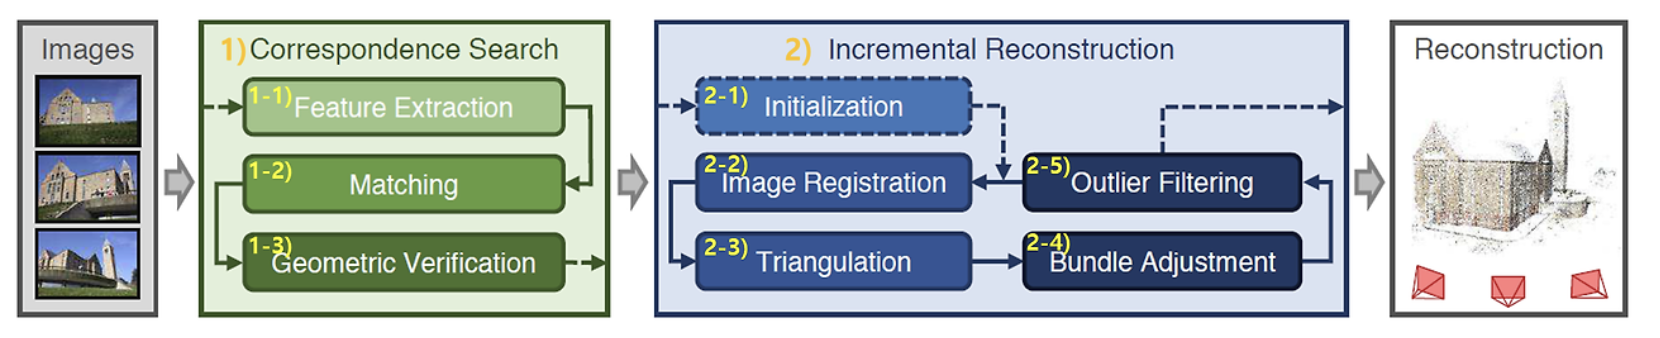
\includegraphics[width=\linewidth]{img/sfm_pipeline.png}
  \caption{Przepływ inkrementalnego SfM}
  \label{fig:sfm_flow}
\end{figure}

\subsubsection{Gaussian Splatting}

Popularną techniką rekonstrukcji z chmury punktów jest siatka (ang. mesh), wykorzystana np. w pracy City3D\cite{city3D}. Często jednak uzyskanie dobrej jakości siatki wymaga kombinacji wielu różnych geometrycznych algorytmów. Wraz z rozwojem sztucznej inteligencji zaczęły pojawiać się i w dziedzinie rekonstrukcji rozwiązania wykorzystujące sieci neuronowe - takie jak np. NeRF\cite{nerf}, gdzie informacje o scenie zawarte są w wagach modelu. Niedoskonałością tego rozwiązania jest jednak długi czas trenowania nawet dla sceny jednego obiektu, wahający się od parunastu godzin do paru dni. Z pomocą przychodzą inne metody, jak np. Gaussian Splatting \cite{gaussiansplatting}, który rezygnuje w całości z sieci neuronowej i wykorzystuje zbiór tzw. "splatów" do zbudowania sceny. Jako że w naszym projekcie stawiamy na optymalne wykorzystanie zasobów, to zdecydowaliśmy się na wybór właśnie ostatniej z wymienionych metod. 

\begin{figure}[!htb]
    % images need to be the same size
    \minipage{0.32\textwidth}
      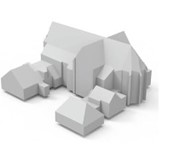
\includegraphics[width=\linewidth]{img/sota/city3dmesh.jpg}
      \caption{City3D - siatka}\label{fig:mesh_example}
    \endminipage\hfill
    \minipage{0.32\textwidth}
      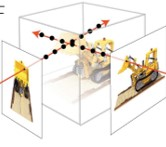
\includegraphics[width=\linewidth]{img/sota/nerfobject.jpg}
      \caption{Nerf - sieć neuronowa}\label{fig:nerf_example}
    \endminipage\hfill
    \minipage{0.32\textwidth}%
      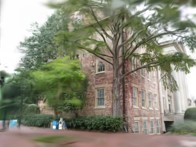
\includegraphics[width=\linewidth]{img/sota/gaussiansplattingobject.jpg}
      \caption{Gaussian Splatting - splat'y}\label{fig:gaussplat_example}
    \endminipage
\end{figure}

Splat (tłum. punkt rozmyty) jest rozszerzeniem punktu i posiada atrybuty
\begin{itemize}
    \item środek (x, y, z)
    \item kolor
    \item przeźroczystość
    \item macierz kowariancji (koduje rotację i skalę)
\end{itemize}

Najlepszy zbiór splatów opisujący scenę jest znajdowany w procesie optymalizacji opisanym poniżej schematem

\begin{figure}[!htb]
    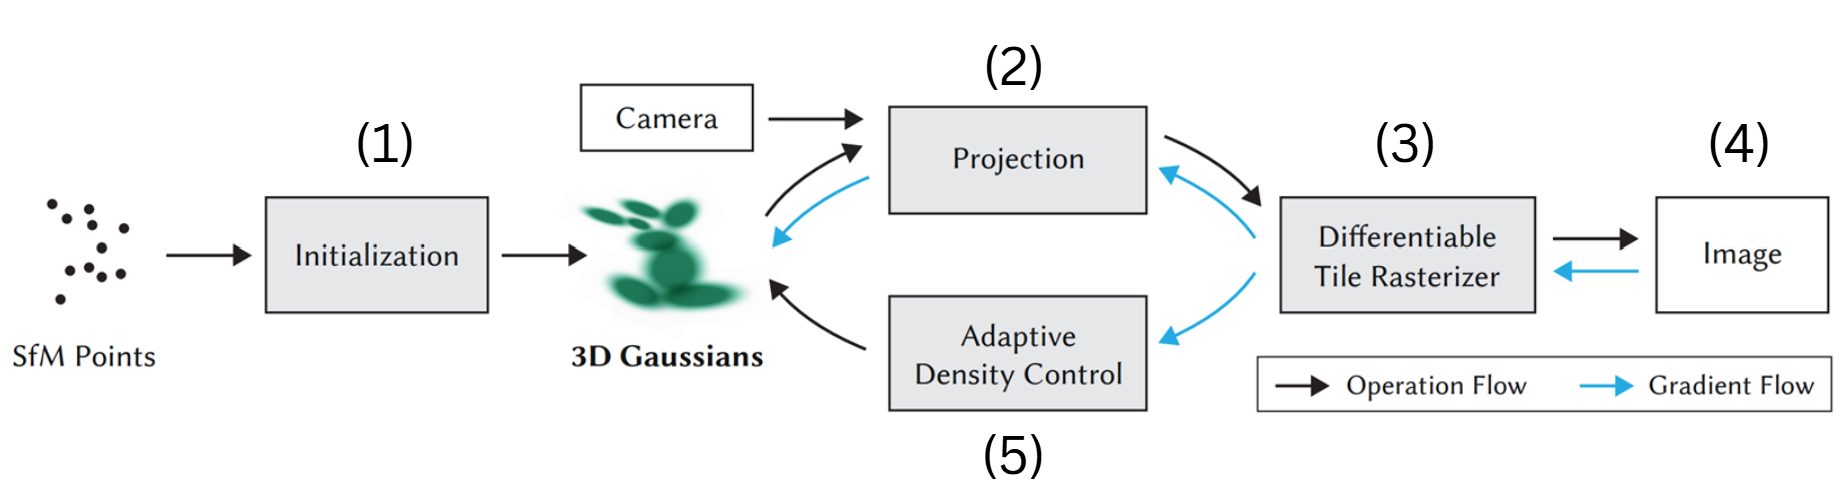
\includegraphics[width=\linewidth]{img/sota/gaussian_splatting_flow.png}
    \caption{Optymalizacja zbioru splatów}\label{fig:splatting_algorithm}
\end{figure}

\begin{enumerate}
    \item Wykorzystanie chmury punktów z rekonstrukcji do inicjalizacji zbioru splatów
    \item Rzutowanie perspektywiczne 3-wymiarowych gaussianów na obraz widziany z danej kamery, czego wynikiem jest zbiór dysków
    \item Renderowanie polegające na akumulowaniu dla każdego piksela wkładu od różnych nachodzących dysków 
    \item Obliczanie funkcji straty - porównanie z prawdziwym obrazkiem z danej kamery
    \item Adaptacja gęstości gaussianów - klonowanie, dzielenie lub usuwanie wg. kryteriów zależnych od strategii
\end{enumerate}

Niestety metoda ta nie pozostaje bez wad. W przypadku dużych zbiorów danych zużycie pamięci może wynieść nawet parę GB, co wymaga dobrej jakości karty graficznej. Inną kwestią jest duża liczba hiperparametrów, które często wymagają ręcznego dostosowania do danej sceny. 

\subsection{Segmentacja semantyczna}

Segmentacja semantyczna jest jednym z zadań uczenia maszynowego zaliczającym się do rodzajów segmentacji. Posiada ona cechy klasyfikacji, polega bowiem na przypisaniu każdemu z punktów w trójwymiarowej chmurze punktów odpowiedniej kategorii semantycznej, \textit{de facto} klasy. Punkty nie są więc traktowane osobno, a łącznie, co umożliwia na rozpoznanie zależności przestrzennych w chmurze punktów. W programie użyto na tym etapie projektu sieci neuronowych, jako rozwiązania szeroko używanego w rozwiązywaniu problemu segmentacji semantycznej obszarów miejskich.

\subsubsection{Architektura}

Istniejące z punktu widzenia architektury wyzwania wynikają ze specyfiki rozpatrywanych danych. Trójwymiarowe chmury punktów są zbiorami nieuporządkowanymi, nierzadko o różnej gęstości punktów w różnych obszarach chmury i różnej wielkości samej chmury. Cechy te wymuszają opracowanie specjalnych architektur adresujących ten problem.

Istniejące architektury sieci neuronowych dla zadania segmentacji semantycznej są przeznaczone głównie dla scen zamkniętych lub pojedynczych obiektów. Popularnym rozwiązaniem jest PointNet\cite{pointnet} oraz jego następca, PointNet++\cite{qi2017pointnetdeephierarchicalfeature} - obydwa oparte na wielowarstwowym perceptronie, jak i również bardziej skomplikowane rozwiązania jak KPConv\cite{thomas2019kpconvflexibledeformableconvolution} implementujące operację konwolucji użyteczną dla trójwymiarowych chmur punktów.

\subsubsection{Zbiór danych}

Ważnym problemem w uczeniu maszynowym jest dobór danych do efektywnego treningu modelu. W opracowywaniu naszego rozwiązania posłużyliśmy się otwartym zbiorem \textit{SensatUrban}\cite{hu2022sensaturban}. Zbiór ten zawiera wiele różnych chmur punktów z obszarami miejskimi w Anglii, o różnej wielkości. Każdemu z punktów przypisana jest jedna z 13 kategorii semantycznych reprezentujacych: podłoże, roślinność, budynek, ścianę, most, parking, tory, drogę, ławkę, samochód, chodnik, rower i obszary wodne. 

\section{Projekt}
\subsection{Specyfikacja wymagań na produkt programowy}
Czy my tu musimy dać diagramy wymagań? :O
Diagram przypadków użycia

\begin{figure}[!htb]
  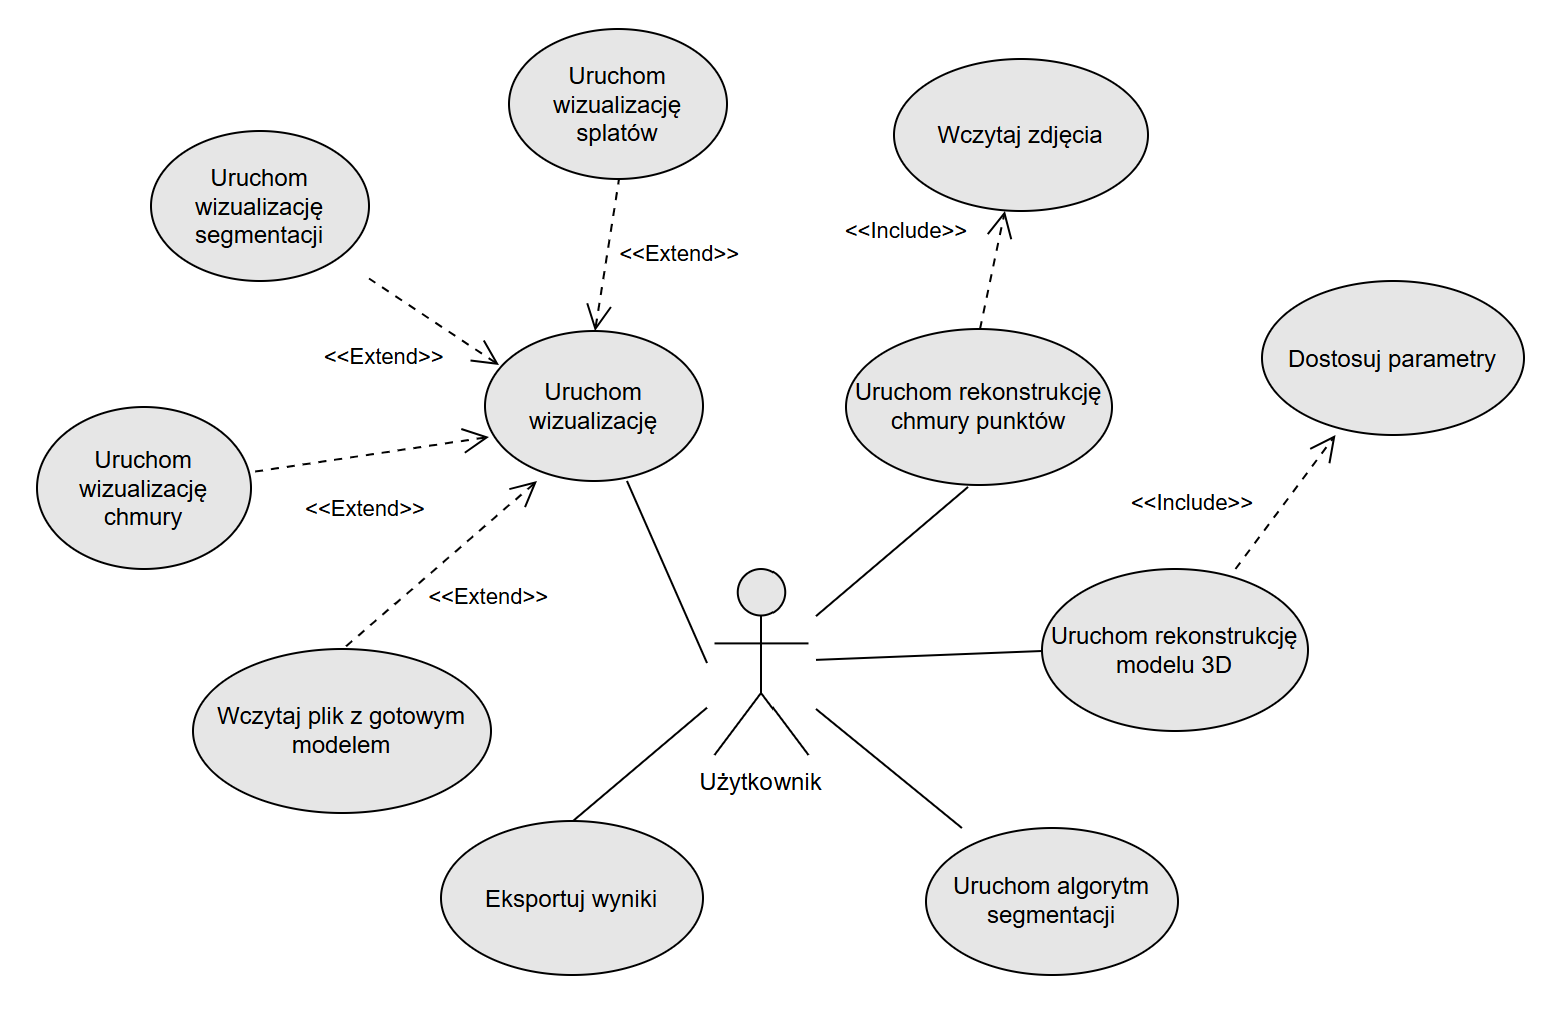
\includegraphics[width=\linewidth]{img/diagram_pu_3.png}
  \caption{Diagram przypadków użycia}\label{fig:use_case_diagram}
\end{figure}

\subsection{Architektura}
Projekt architektury, zastosowane wzorce projektowe???
Jakiś język graficzny tutaj

\subsection{Implementacja}
Opis zastosowanych technologii i dokumentów

\subsubsection{Struktura plikowa projektu}

to wrzucić pod implementację

% millon opcji https://tex.stackexchange.com/questions/5073/making-a-simple-directory-tree
\begin{forest}
  for tree={
    grow'=0,
    child anchor=west,
    parent anchor=south,
    anchor=west,
    calign=first,
    edge path={
      \noexpand\path [draw, \forestoption{edge}] (!u.south west) ++(3pt,0) -- +(-3pt,0) |- (.child anchor)\forestoption{edge label};
    },
    before typesetting nodes={
      if n=1
        {insert before={[,phantom]}}
        {}
    },
    fit=band,
    before computing xy={l=15pt},
  }
[project
  [src
    [urb3d
      [rendering]
      [geometry]
      [models]
      [splats]
    ]
  ]
  [docs
    [main.pdf]
    [readme.txt]
  ]
  [config
    [config.json]
  ]
  [data
  [city\_model
        [images]
        [sparse
            [images.bin]
            [cameras.bin]
            [points.bin]
        ]
        [model.pt]
        [model.ply]
        [segmentation.ply]
    ]
  ]
]
\end{forest}

\subsubsection{Structure from motion}
Jedną z funkcjonalności oferowanych przez przygotowane oprogramowanie jest wyznaczanie struktury przestrzennej sceny w postaci chmury punktów na podstawie zbioru fotogramów przy pomocy techniki Structure from motion. Zaproponowana implementacja opiera się na wykorzystaniu popularnego narzędzia COLMAP, które zostało włączone do projektu w postaci pythonowej biblioteki \textit{pycolmap}. Biblioteka ta oferuje szereg funkcji umożliwiających przeprowadzenie kluczowych etapów procesu SfM, w tym wykorzystane w projekcie funkcjonalności do wykrywania cech charakterystycznych na obrazach, dopasowywania punktów wspólnych między obrazami czy przeprowadzania inkrementalnej rekonstrukcji, która dodatkowo została skonfigurowana za pomocą parametrów dobranych tak, aby zapewnić zadowalającą jakość wyniku przy zachowaniu wydajności.

W wyniku działania tak zaimplementowanego procesu powstają pliki binarne zapisujące dane przede wszystkim wyznaczonych punktów 3D i pozycji kamer. Biblioteka \textit{pycolmap} umożliwiła dodatkowo łatwe wprowadzenie funkcjonalności eksportu wyników do formatu PLY, którego to formatu plik zostaje wykorzystany do wizualizacji wygenerowanej chmury punktów. Z kolei reprezentacja w postaci plików binarnych zostaje w kolejnych etapach wczytywana i po przefiltrowaniu służy za podstawę do modelowania z zastosowaniem algorytmu Gaussian Splatting.

\begin{figure}[!ht]
  \centering
  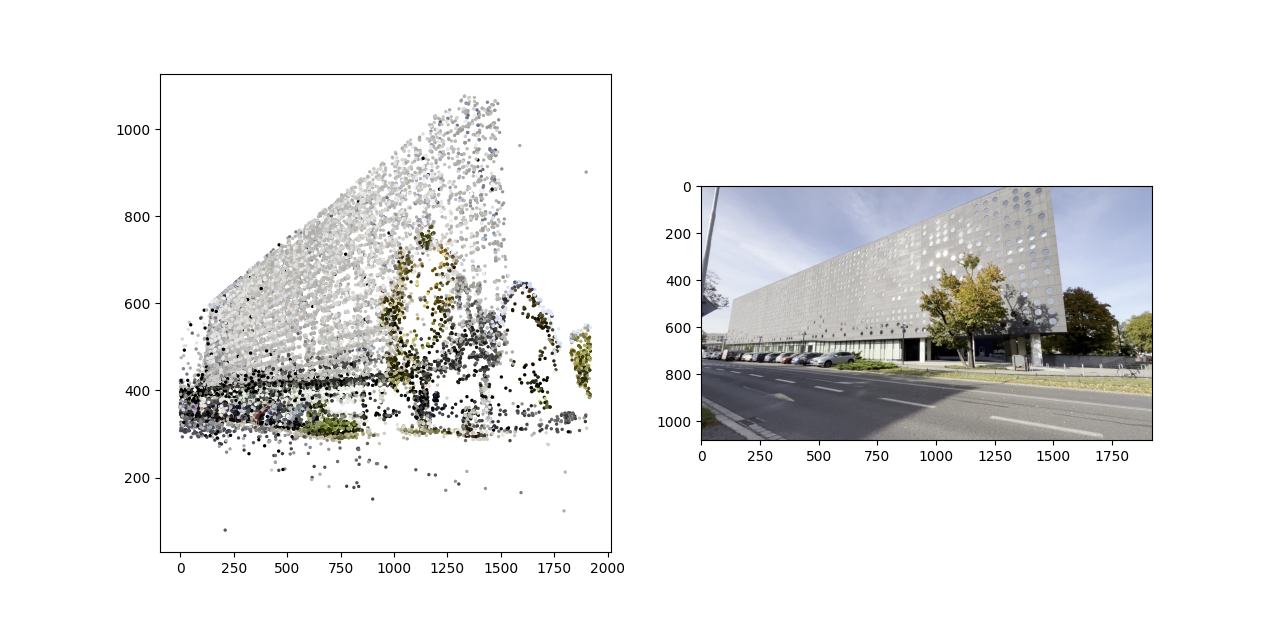
\includegraphics[width=0.9\linewidth]{img/sfm_projection.png}
  \caption{Projekcja przykładowej chmury punktów na płaszczyznę porównana do zdjęcia}
\end{figure}

\subsubsection{Filtracja chmury punktów}
Ważny i wpływający na jakość wynikowej rekonstrukcji element przetwarzania chmury punktów jakim jest jej filtracja pojawia się na dwóch etapach projektu: po przeprowadzeniu generacji chmury punktów i przed uruchomieniem algorytmu segmentacji. 

Celem filtracji, która ma miejsce bezpośrednio po wygenerowaniu chmury punktów, a przed uruchomieniem algorytmu Gaussian Splatting jest usunięcie szumów. Pozwoli ono na poprawę reprezentacji danych wejściowych do algorytmu oraz redukcję liczby punktów nieistotnych, co ważne jest w kontekście optymalizacji zapotrzebowania na zasoby obliczeniowe.

Przy implementacji tego elementu wykorzytano funkcjonalność statystycznego usuwania punktów odstających (\textit{ang. statistical outlier removal}) oferowaną przez szeroko stosowaną w przetwarzaniu danych przestrzennych bibliotekę Open3D. Metoda ta analizuje lokalną gęstość punktów na podstawie wybranej liczby sąsiadów. Z wykorzystaniem ustalanego progu związanego z odchyleniem standardowym średnich odległości w chmurze punktów, odrzucane są punkty, które znajdują się dalej od swoich sąsiadów w porównaniu do średniej dla chmury. 

Filtracja chmury punktów przed segmentacją ma za zadanie eliminację punktów, które znajdują się 
statystycznie dalej od centralnego obszaru chmury, co pozwoli na ograniczenie jej do bardziej zwartej struktury. W ramach tej filtracji zaimplementowano metodę, która początkowo określa zakres, wyznaczając dla każdej współrzędnej pierwszy kwartyl \textit{Q1}, trzeci kwartyl \textit{Q3} i rozstęp międzykwartylowy $IQR = Q1 - Q3$. Na ich podstawie obliczane są z użyciem parametru $\alpha$ granice zakresu: $Q1 - \alpha * IQR$ i $Q3 + \alpha * IQR$. Odrzucane zostają punkty, dla których wartość którejkolwiek ze współrzędnych znajduje się poza wyznaczonym zakresem.


\subsubsection{Gaussian Splatting}
W celu uruchomienia algorytmu Gaussian Splatting korzystamy z gotowej implementacji którą 
zapewnia biblioteka \href{https://docs.gsplat.studio/main/index.html}{\textit{gsplat}} \cite{ye2024gsplatopensourcelibrarygaussian}. Znajdują się w niej metody które odzwierciedlają wykonywane kroki w teoretycznym opisie algorytmu (np. \textit{rasterization}) a także dodatkowe elementy oparte na nowszych badaniach które usprawniają proces trenowania i renderowania (np. \textit{sparse gradient}, \textit{absgrad}, itp.). Dodatkowym plusem biblioteki jest wsparcie do renderowania dużych scen. Jej użycie wymaga posiadania karty graficznej CUDA.  

Jedną z naszych kontrybucji jest dostosowanie istniejącego skryptu trenującego \href{https://github.com/nerfstudio-project/gsplat/blob/main/examples/simple_trainer.py}{simple\_trainer} tak aby działał on poprawnie i zgodnie z naszymi wymaganiami. Przyjmuje on następujące argumenty:

% change style to not highlight python specific words
\lstset{style=basicstyle}
\begin{lstlisting}[language=SHELXL] 
  options:
  -h, --help            show this help message and exit
  --data_dir DATA_DIR   Path to the data directory.
  --result_dir RESULT_DIR
                        Path to the results directory.
  --data_factor DATA_FACTOR
                        Data factor.
  --init_type {sfm,random}
                        Initialization type.
  --strategy {default,mcmc}
                        Strategy type.
  --max_steps MAX_STEPS
                        Maximum number of steps.
  --init_num_pts INIT_NUM_PTS
                        Initial number of points (only for random).
  --delta_steps DELTA_STEPS
                        Delta steps for evaluation and saving.
  --scale_reg SCALE_REG
                        Scale regularization value.
  --opacity_reg OPACITY_REG
                        Opacity regularization value.
  --min_opacity MIN_OPACITY
                        Minimum opacity.
  --refine_stop_iter REFINE_STOP_ITER
                        Refinement stop iteration.
  --refine_every REFINE_EVERY
                        Refine frequency (iterations).
  --refine_start_iter REFINE_START_ITER
                        Refinement start iteration.
  --reset_every RESET_EVERY
                        Reset opacities every this steps. [strategy=default]
  --pause_refine_after_reset PAUSE_REFINE_AFTER_RESET
                        Pause refining GSs until this number of steps after reset. [strategy=default]
  --cap_max CAP_MAX     Maximum cap for MCMC gaussians. [strategy=mcmc]
  --sh_degree_interval SH_DEGREE_INTERVAL
                        Add spherical harmonics degree interval.
  --sh_degree {1,2,3}   Degree of spherical harmonics.
  --init_scale INIT_SCALE
                        Initial scale.
  --init_opa INIT_OPA   Initial opacity.
  --packed PACKED       Use packed mode for rasterization.
  --sparse_grad SPARSE_GRAD
                        Use sparse gradients for optimization.
\end{lstlisting}

\lstset{style=pythonstyle}

Z których obowiązkowe to \textit{data\_dir} - ścieżka do folderu z rekonstrukcją i zdjęciami i \textit{result\_dir} - ścieżka gdzie zostaną zapisane wyniki. 

\textbf{Opis parametrów}
\begin{itemize}
  \item \textit{data\_dir} - obowiązkowy; ścieżka do folderu z rekonstrukcją i zdjęciami
  \item \textit{result\_dir} - obowiązkowy; ścieżka gdzie zostaną zapisane wyniki
  \item init\_type - sposób inicjalizacji chmury punktów, losowy (random) lub z rekonstrukcji sfm (sfm)
  \item strategy - strategia zagęszczania gaussianów
  \item max\_steps - maksymalna liczba iteracji
  \item init\_num\_pts - początkowa liczba punktów dla sposobu inicjalizacji random
  \item delta\_steps - liczba iteracji po którch dokonywać ewaluacji oraz zapisu checkpointa
  \item scale\_reg - współczynnik regularyzacji skali gaussianów
  \item opacity\_reg - współczynnik regularyzacji przeźroczystości gaussianów
  \item min\_opacity - prog przeźroczystości poniżej którego splaty są odrzucane
  \item refine\_every - liczba iteracji po których następuje ulepszanie gaussianów wg. wybranej strategii 
  \item refine\_start\_iter - liczba iteracji od początku trenowania po której zachodzi pierwszy raz ulepszanie
  \item reset\_every - liczba iteracji po której zachodzi wyzerowanie przeźroczystości jeśli strategią jest \textit{default}
  \item pause\_refine\_after\_reset - liczba iteracji po wyzerowaniu które należy odczekać aby zaszedł krok doskonalenia gaussianów jeśli strategią jest \textit{default}
  \item cap\_max - maksymalna liczba gaussianów jeśli strategią jest \textit{mcmc}
  \item sh\_degree\_interval - liczba iteracji po której dodawany jest kolejny stopień zmiennych harmonicznych
  \item sh\_degree - stopień współczynników zmiennych harmonicznych 
  \item init\_scale - początkowa skala gaussianów 
  \item init\_opa - początkowa przeźroczystość gaussianów
\end{itemize}

\section{Wyniki}

\subsection{Specyfikacja wymagań na produkt programowy}

\begin{figure}[!htb]
    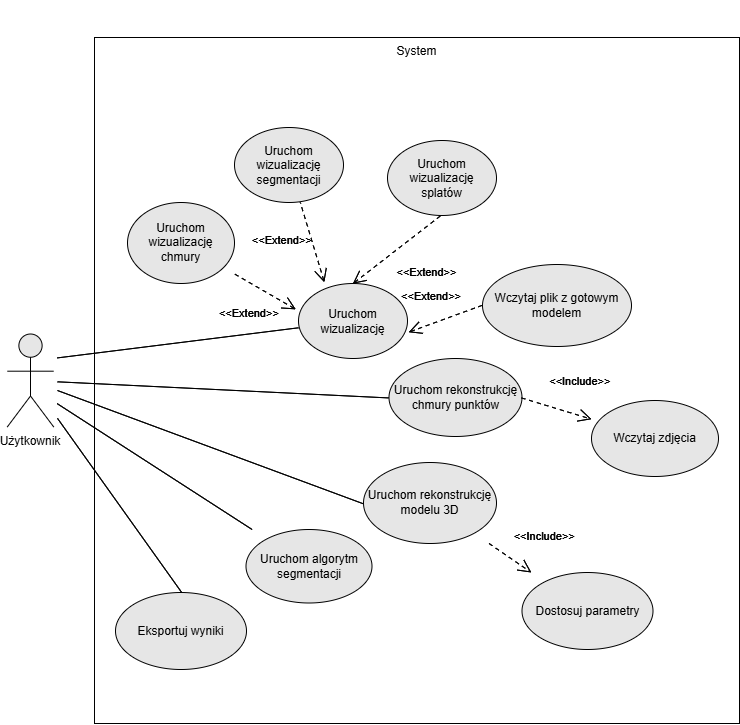
\includegraphics[width=1.0\linewidth]{img/diagramy/zpi use case.png}
    \caption{Diagram przypadków użycia}\label{fig:use_case_diagram}
  \end{figure}

\clearpage

\subsection{Architektura}

\begin{figure}[!htb]
    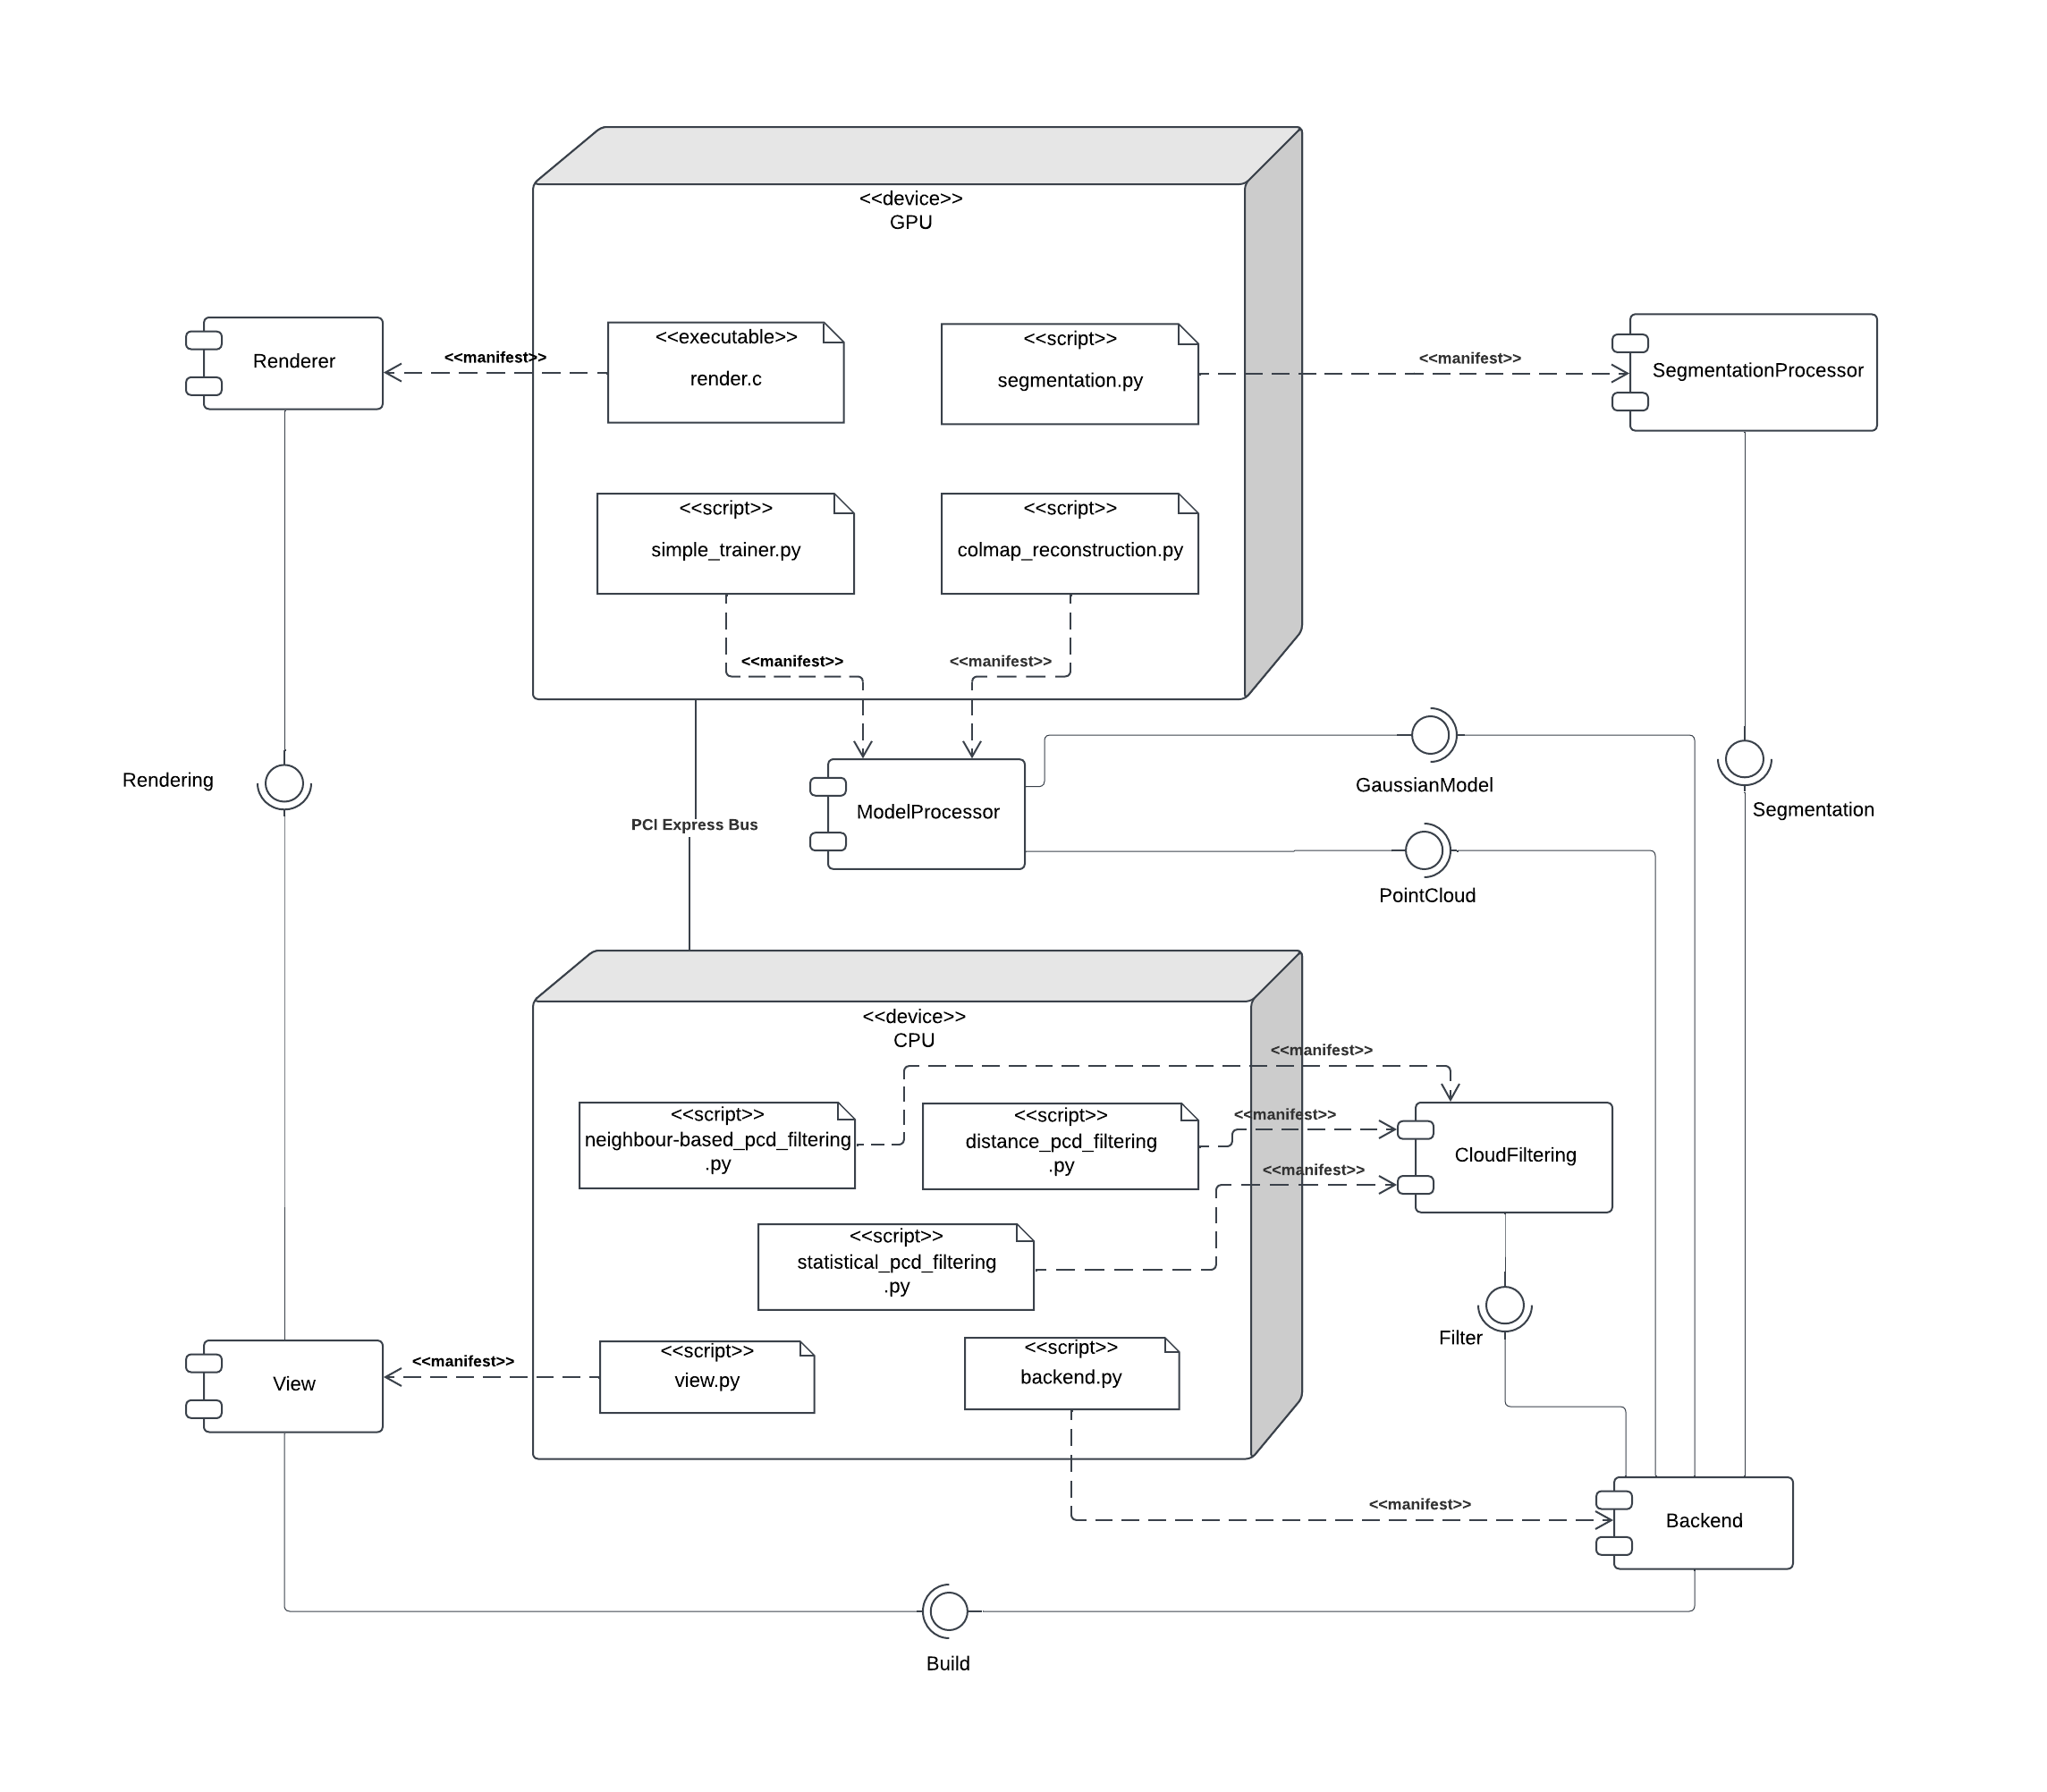
\includegraphics[width=1.0\linewidth]{img/diagramy/diagram_wdrozenia_komponentow_3.png}
    \caption{Diagram wdrożenia komponentów}\label{fig:components_diagram}
\end{figure}

\subsubsection{Architektura}
Projekt został zrealizowany w oparciu o wzorzec projektowy \textbf{MVVM} (Model-View-ViewModel), który został odpowiednio dostosowany do specyfiki aplikacji w celu zapewnienia modularności oraz uproszczenia procesu modyfikacji i rozbudowy.

\textbf{Adaptacja wzorca MVVM}
\begin{figure}[h!]
    \centering
    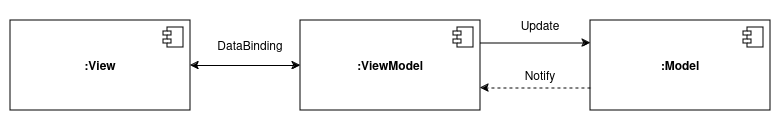
\includegraphics[width=0.8\textwidth]{img/diagramy/architektura.png}
    \caption{Schemat zaadaptowanego wzorca MVVM w projekcie.}
\end{figure}

W zaimplementowanym rozwiązaniu wzorzec \textbf{MVVM} został zmodyfikowany w celu optymalizacji komunikacji między komponentami aplikacji. Dzięki temu możliwe było osiągnięcie spójności architektury oraz jej wysokiej skalowalności.

\paragraph{Opis komponentów architektury}
\begin{figure}[h!]
    \centering
    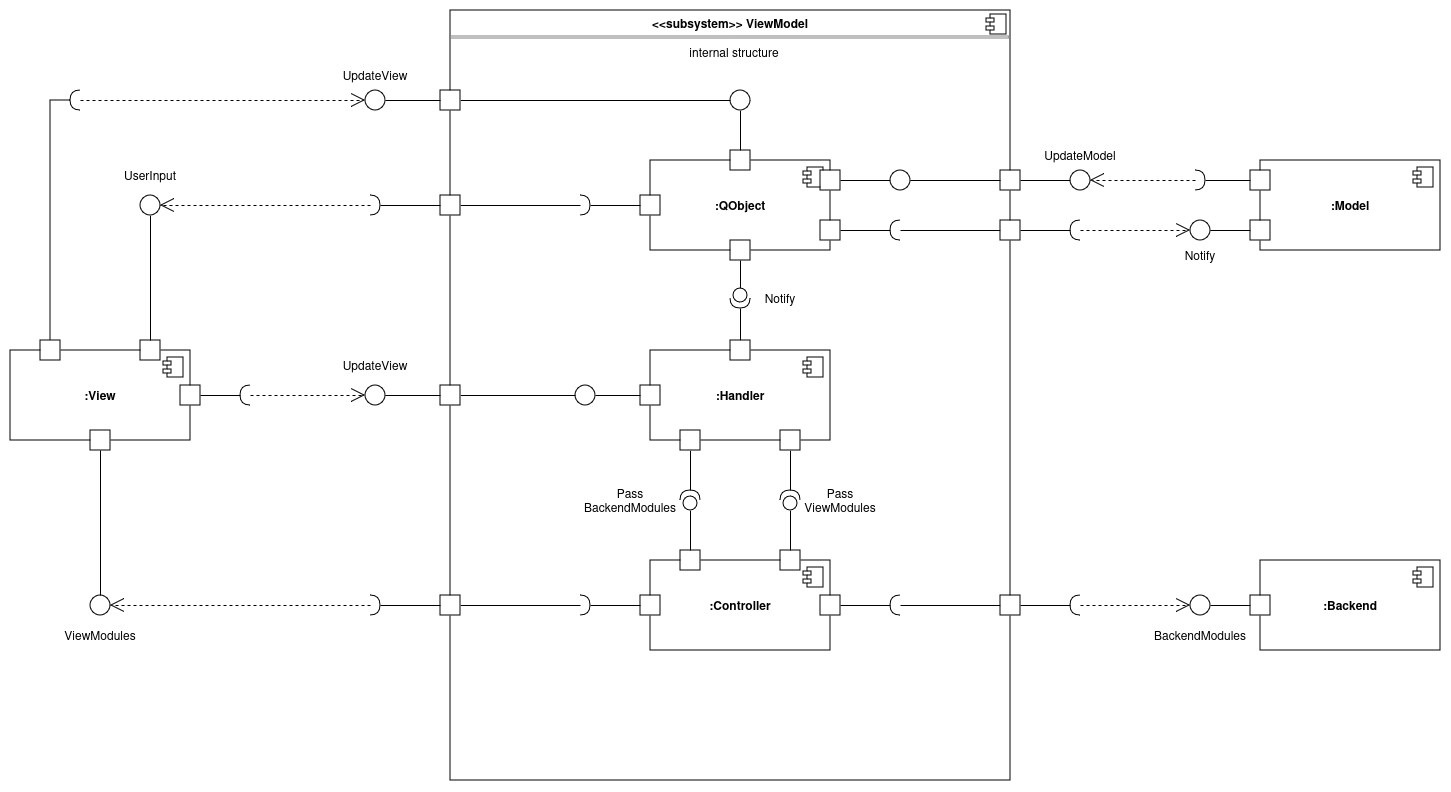
\includegraphics[width=0.8\textwidth]{img/diagramy/diagram_komp_vm.png}
    \caption{Struktura komponentów ViewModel w projekcie.}
\end{figure}

W projekcie klasa \texttt{ViewModel} zastępuje tradycyjny zbiór klas, takich jak:
\begin{itemize}
    \item \texttt{Controller} -- odpowiadający za sterowanie logiką,
    \item \texttt{QObject} -- obsługujący komunikację z frontendem,
    \item \texttt{Handler} -- integrujący dodatkowe funkcjonalności wizualne.
\end{itemize}

\textbf{Rola \texttt{QObject}}
Klasa \texttt{QObject} pełni funkcję tradycyjnego komponentu \texttt{ViewModel}, umożliwiając komunikację między warstwą logiki a frontendem aplikacji. Wykorzystuje mechanizm sygnałów dostarczany przez bibliotekę PyQt, co pozwala dynamicznie informować widok o zmianach stanu aplikacji.

\textbf{Handler jako rozszerzenie funkcjonalności}
\texttt{QObject} został wzbogacony o klasę \texttt{Handler}, która pozwala na łatwą implementację funkcji wizualnych w już istniejącej architekturze. Dzięki temu projekt zachowuje przejrzystość i elastyczność.

\textbf{Integracja za pomocą \texttt{Controller}}
Klasy \texttt{QObject} i \texttt{Handler} są zintegrowane za pomocą \texttt{Controller}, który zapewnia jednolity interfejs oraz ułatwia zarządzanie komponentami aplikacji.

Na diagramie widoczny jest dodatkowy komponent \textbf{Backend}, będący zbiorem skryptów, które dostarczają interfejs dla wymaganej funkcjonalności aplikacji. Backend odpowiada za obsługę logiki niezwiązanej bezpośrednio z widokiem oraz wspiera pozostałe komponenty architektury, zapewniając większą modularność.

\paragraph{Zalety wdrożonego rozwiązania}
Przedstawione rozwiązanie zapewnia następujące korzyści:
\begin{itemize}
    \item \textbf{Modularność} -- możliwość łatwego dodawania i modyfikowania komponentów bez ingerencji w istniejącą strukturę.
    \item \textbf{Skalowalność} -- umożliwia rozbudowę aplikacji o nowe funkcjonalności przy zachowaniu spójności architektury.
    \item \textbf{Wsparcie dla współbieżności} -- dzięki zastosowaniu mechanizmu sygnałów PyQt implementacja współbieżności jest intuicyjna i efektywna.
\end{itemize}

\paragraph{Podsumowanie}
Zaimplementowany wzorzec MVVM, w połączeniu z dodatkowymi modyfikacjami, pozwolił osiągnąć elastyczną i skalowalną architekturę aplikacji. Dzięki zastosowanemu podejściu projekt spełnia założenia modularności, umożliwiając łatwą rozbudowę oraz utrzymanie w przyszłości.

% \subsection{Implementacja}

\subsection{Wizualizacja}
W celu zapewnienia użytkownikowi końcowemu zintegrowanego i spójnego środowiska wizualizacji całego procesu – od wgrania plików wejściowych po interakcję z modelem – zaprojektowano od podstaw interfejs oraz system renderowania.

Założeniem projektu była implementacja intuicyjnego, dynamicznego i responsywnego \textbf{interfejsu}[\ref{fig:ui}] przy pomocy biblioteki \textit{PyQt} oraz języka \textit{QML}. Interfejs został zintegrowany z wydajnym systemem \textbf{renderingu}[\ref{fig:rendering}] GPU, wykorzystującym technologie \textit{OpenGL}, \textit{OpenCL} oraz język \textit{C}. Dodatkowo, użytkownik ma możliwość alternatywnego renderowania z wykorzystaniem biblioteki \textit{VisPy}.

Projekt rozwiązuje problem fragmentaryczności funkcji dostępnych w innych aplikacjach, oferując spójne środowisko do obsługi modeli 3D, obejmujące procesy tworzenia, modyfikacji, segmentacji oraz wizualizacji danych.
\\[10pt]
\textbf{Funkcjonalności interfejsu}

\begin{itemize} \item wybór zdjęć, \item ustawienie parametrów, \item generowanie chmury punktów, \item generowanie splatów, \item segmentacja splatów, \item wizualizacja wyników. \end{itemize}

\vspace{10pt}
{\setlength{\parindent}{0pt}
\textbf{Rendering}
}

Rendering wykorzystuje plik .ply jako dane wejściowe do wczytania splatów. Splaty te są reprezentowane przez sześciany z dodatkowymi parametrami przechowywanymi w Shader Storage Buffer Object (SSBO), co umożliwia efektywny odczyt dużych ilości danych. Takie podejście jest szczególnie przydatne w przypadku scen zawierających nawet do dwóch milionów obiektów.

Do przechowywanych parametrów należą: \begin{itemize} \item pozycja, \item skala, \item rotacja, \item kolor, \item przezroczystość. \end{itemize}

Podczas procesu renderowania, model sześcianu jest odpowiednio przekształcany na podstawie tych parametrów, co pozwala na uzyskanie splatów na wyjściu. Takie podejście umożliwia abstrakcyjne definiowanie splatów przy jednoczesnym zachowaniu wysokiej dokładności wizualnej.

\clearpage

\begin{figure}[!ht]
    \centering
    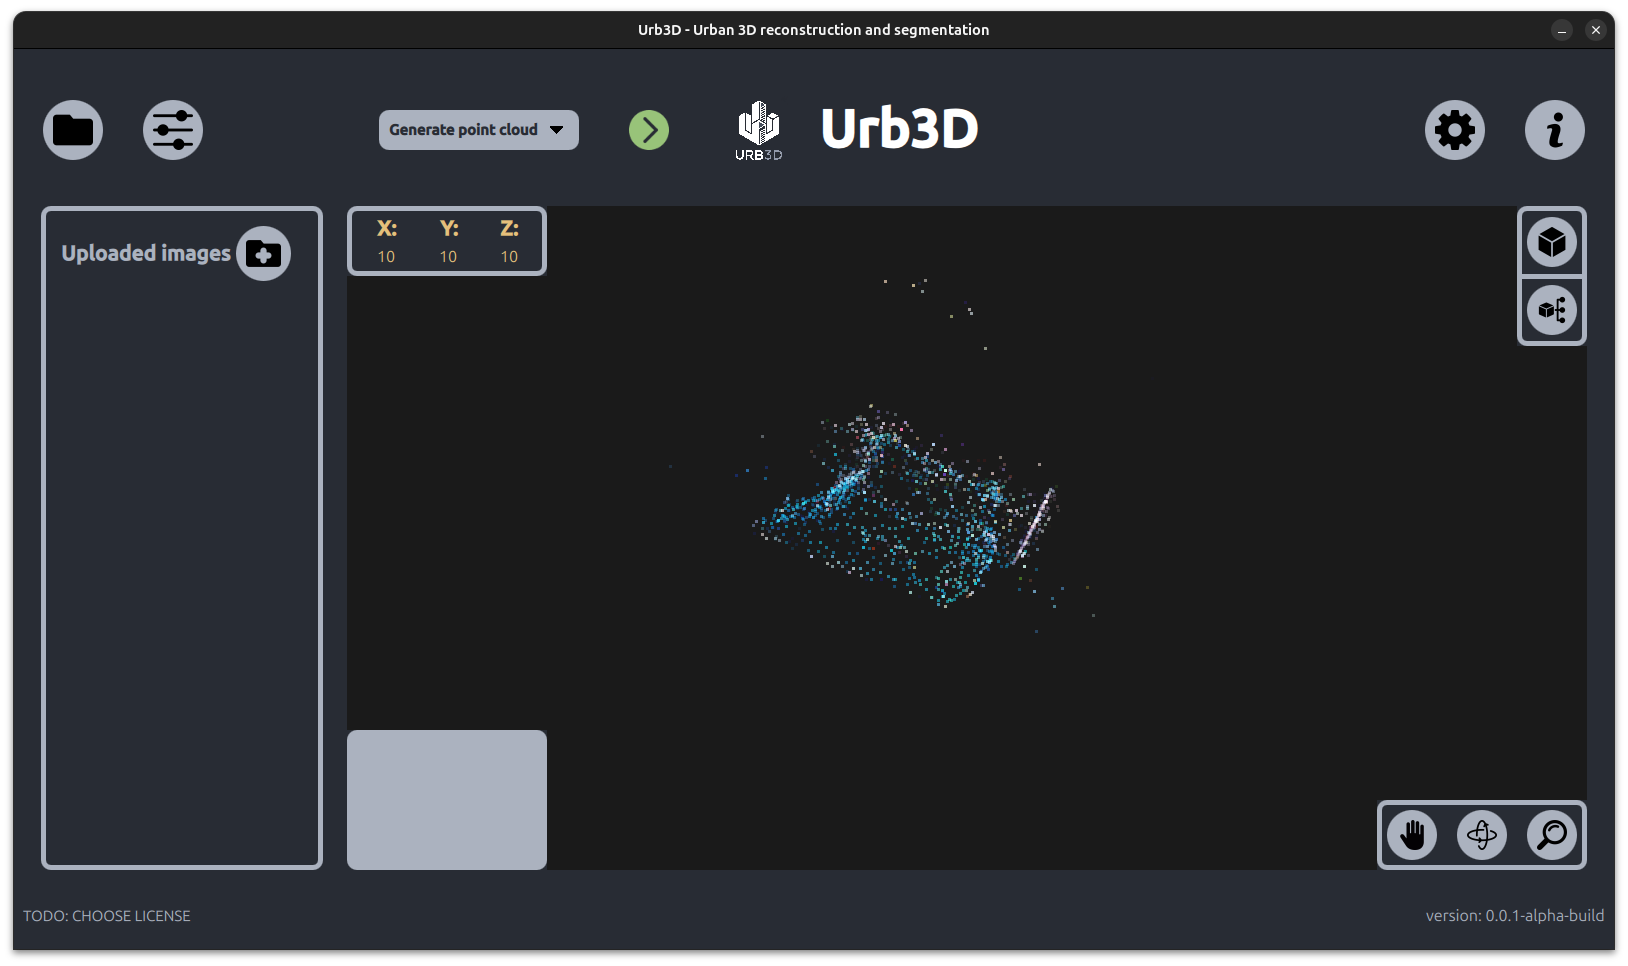
\includegraphics[width=\textwidth]{images/UI-Rendering.png}
    \caption{Zrzut ekranu przedstawiający główny widok aplikacji}
    \label{fig:ui}
\end{figure}

\begin{figure}[!ht]
    \centering
    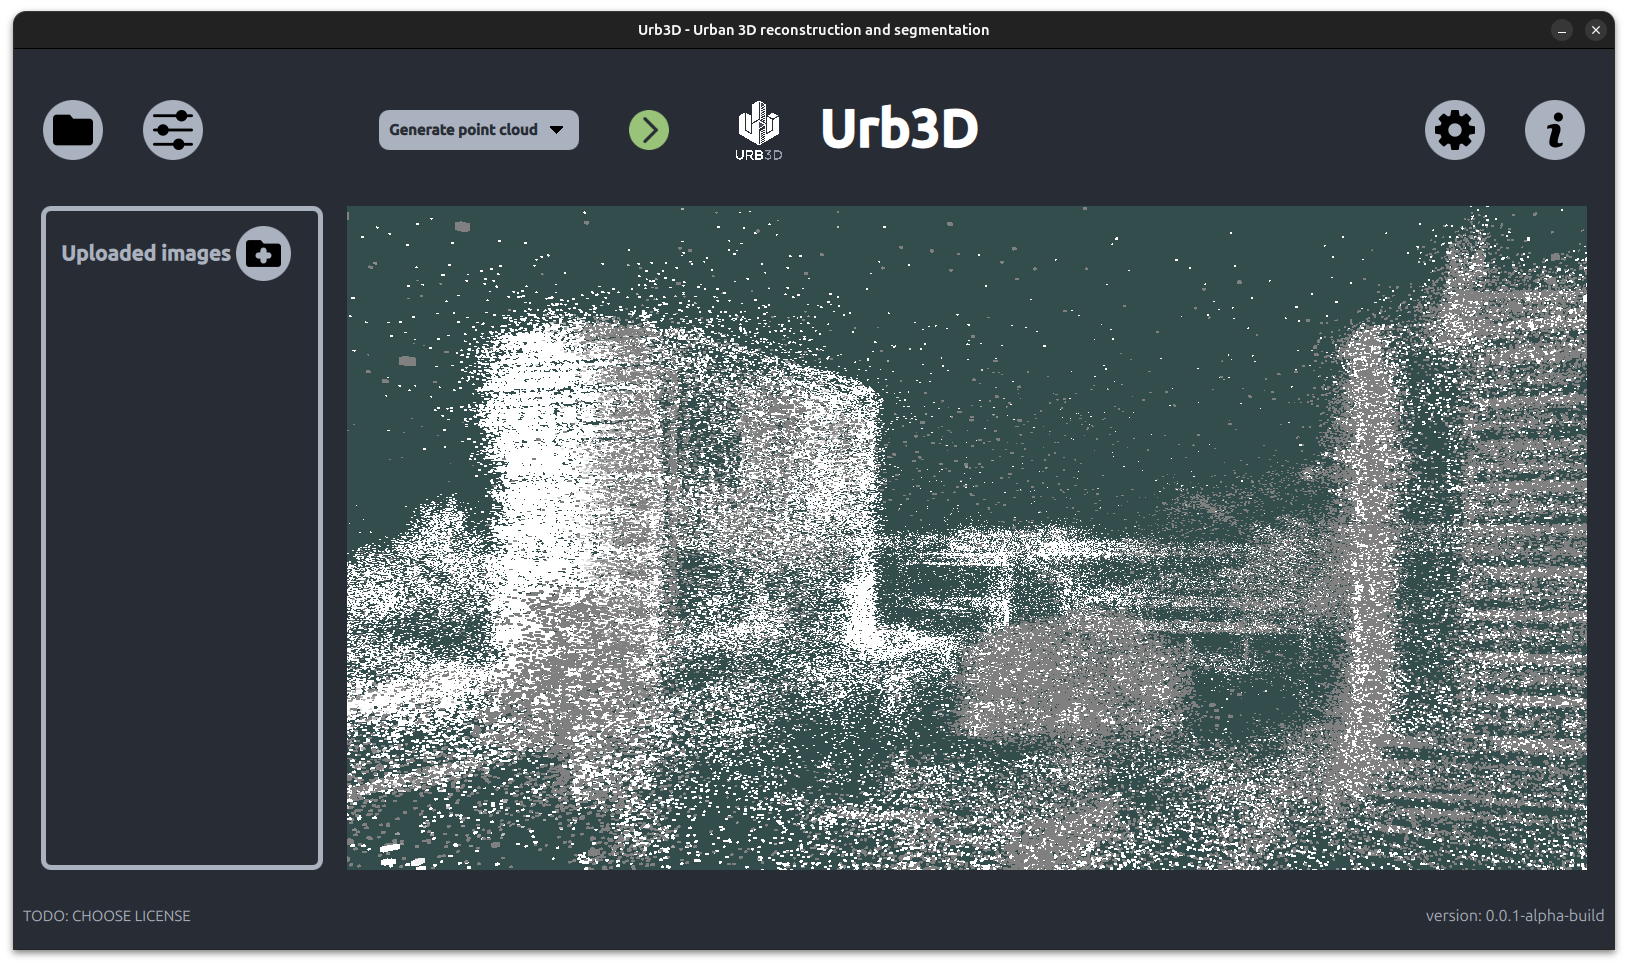
\includegraphics[width=\textwidth]{images/cloud_rendering.png}
    \caption{Zrzut ekranu przedstawiający własny renderer}
    \label{fig:rendering}
\end{figure}

\subsection{Rendering}

W aplikacji zaimplementowano autorski system renderingu w celu zapewnienia wysokiej wydajności oraz wygody użytkowania przez użytkownika końcowego. Do realizacji tego rozwiązania wykorzystano język C oraz bibliotekę OpenGL z rozszerzeniami GLEW, GLFW i CGLM.

\begin{figure}[h!]
    \centering
    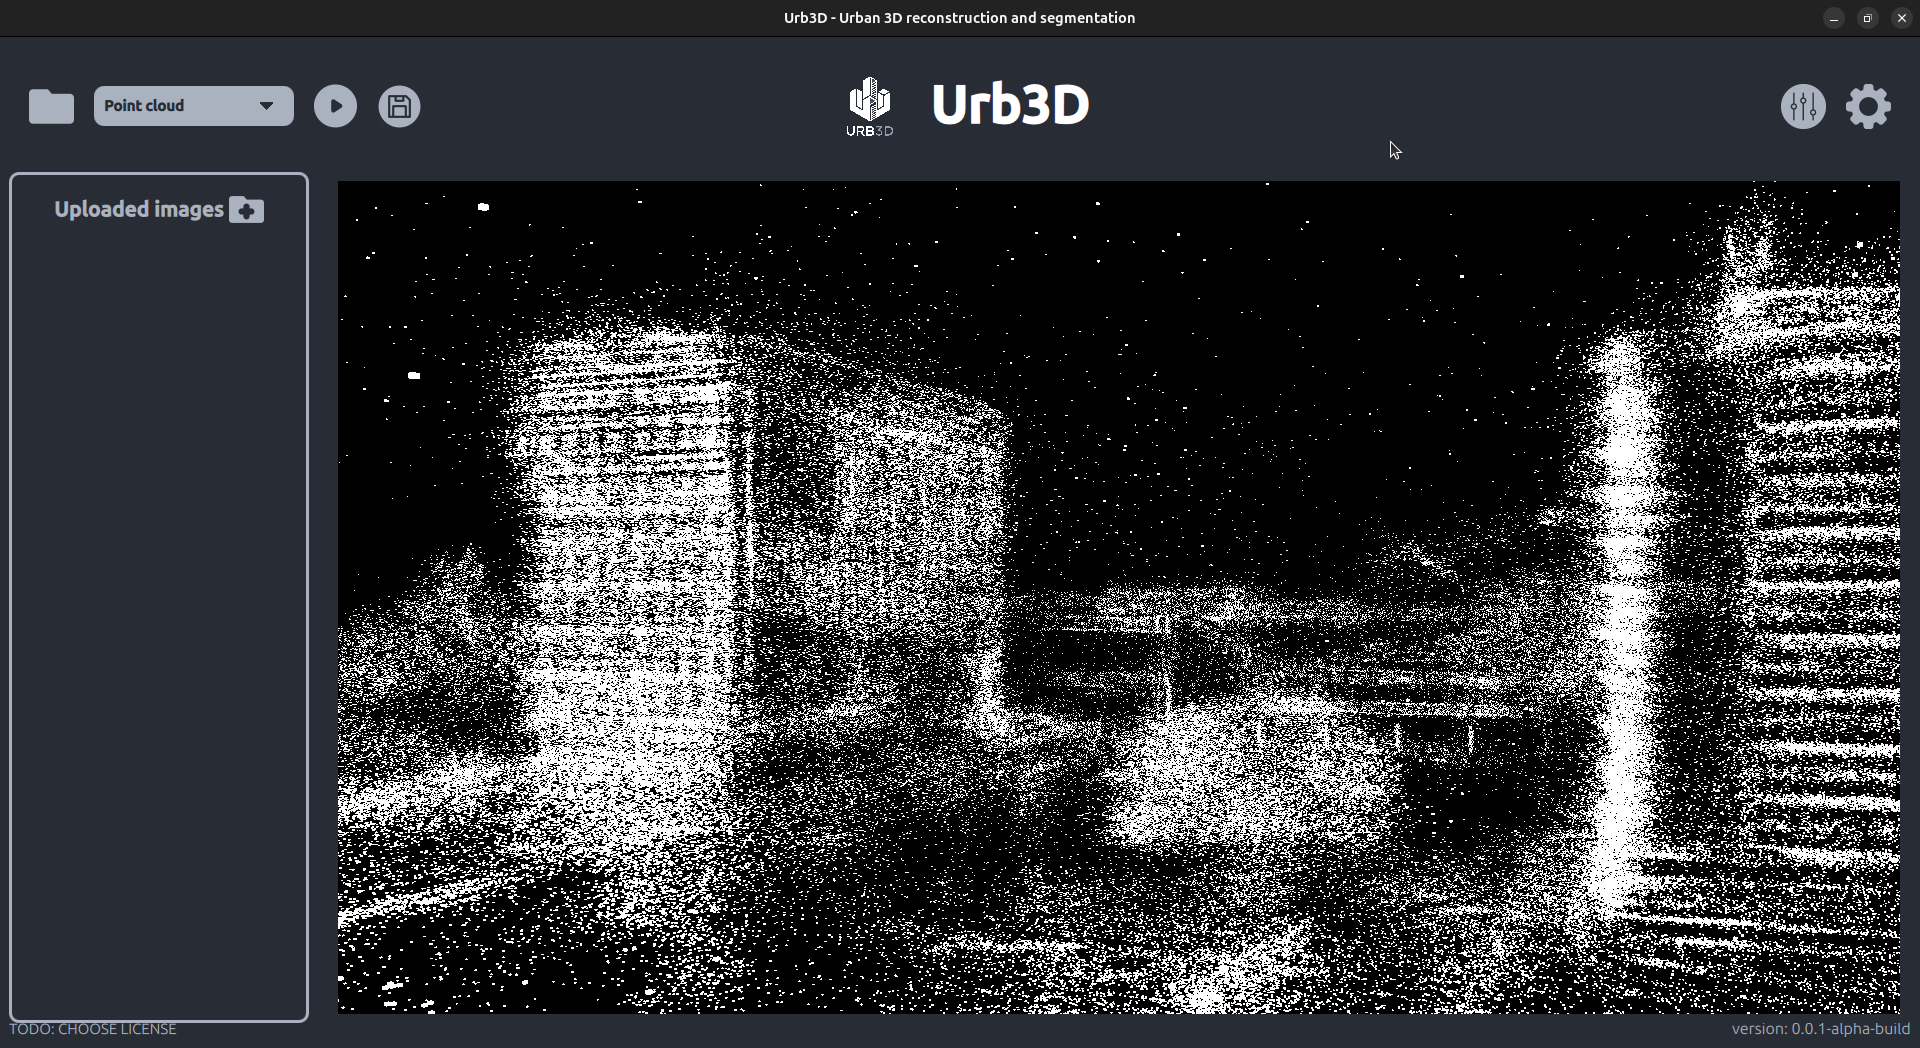
\includegraphics[width=0.8\textwidth]{img/wizualizacja/ui_rendering.png}
    \caption{Widok główny aplikacji z zaimplementowanym renderingiem.}
    \label{fig:widok_glowny}
\end{figure}

\subsubsection{Integracja z Pythonem}
Rendering został udostępniony jako dynamiczna biblioteka współdzielona, co umożliwia jego integrację z aplikacjami napisanymi w języku Python. Dzięki temu, w połączeniu z frameworkiem PyQt, rendering może być efektywnie wykorzystywany w aplikacjach graficznych.

\begin{figure}[h!]
    \centering
    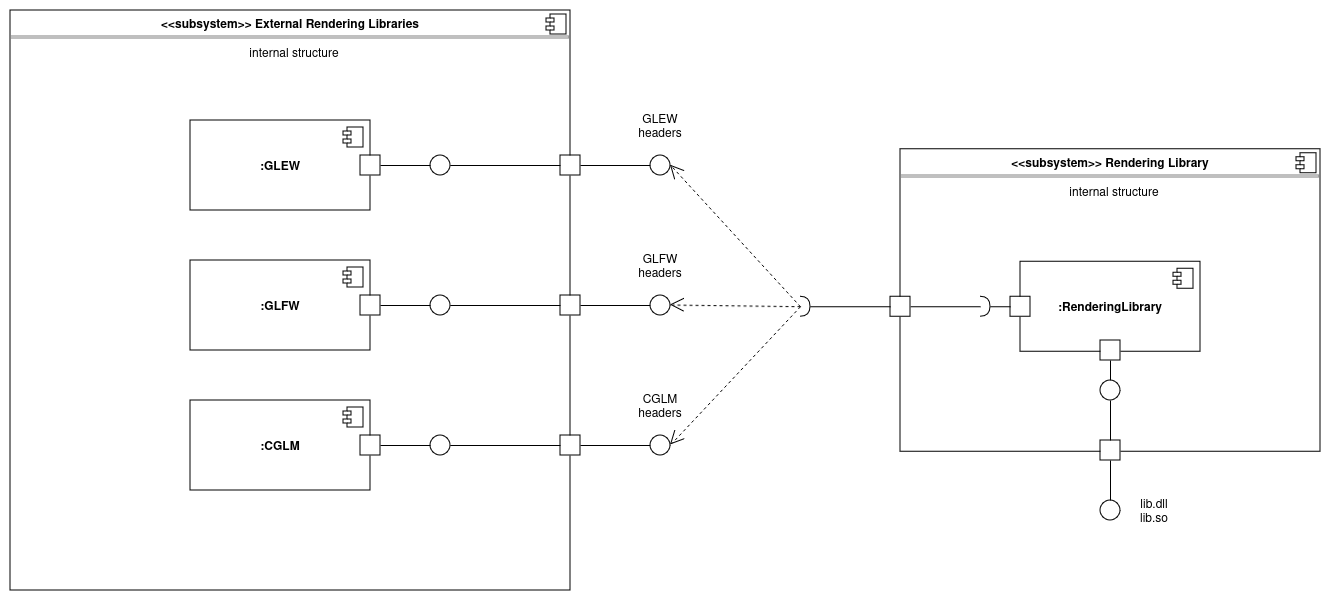
\includegraphics[width=0.8\textwidth]{img/diagramy/diagram_komp_rendering.png}
    \caption{Diagram przedstawiający architekturę integracji renderingu z Pythonem.}
    \label{fig:diagram}
\end{figure}

\subsubsection{Implementacja systemu renderingu}

\textbf{Reprezentacja punktów i splatów}
Wizualizacja punktów oraz splatów została zrealizowana za pomocą sześcianów, które są skalowane i rotowane w taki sposób, aby przypominały elipsoidy. Przetworzone w ten sposób sześciany są następnie renderowane przy użyciu shaderów, co pozwala na uzyskanie efektu ich zaokrąglenia.

\textbf{Optymalizacja wydajności}
Aby zwiększyć wydajność obliczeń graficznych, wykorzystano GPU z użyciem obiektów SSBO (Shader Storage Buffer Objects). SSBO umożliwiają przechowywanie i przetwarzanie dużych ilości danych bezpośrednio na karcie graficznej, co minimalizuje obciążenie procesora głównego.

\clearpage

W ramach procesu renderingu wczytywane są dane statyczne dla domyślnego sześcianu, a następnie przetwarzane są atrybuty poszczególnych punktów, takie jak:
\begin{itemize}
    \item pozycja,
    \item skalowanie,
    \item rotacja,
    \item przezroczystość,
    \item kolor.
\end{itemize}

Takie podejście zapewnia elastyczność oraz wysoką wydajność w generowaniu scen 3D.

% \clearpage

\subsection{Technologie}

W projekcie wykorzystano następujące technologie

\begin{itemize}
    \item \textbf{C/C++}: OpenCL, OpenGL
    \item \textbf{Python}: Pytorch, pycolmap, open3d, pyvista, PyQt (numpy, matplotlib), pytest
    \item CloudCompare, Meshlab
    \item \textbf{GPU}
    \item Jira, Confluence, Github, Discord
\end{itemize}

\begin{figure}[!ht]
    \centering
    
\includegraphics[width=0.9\linewidth]{img/sota/technologie.png}
  \end{figure}

\subsubsection{Struktura plikowa projektu}

% millon opcji https://tex.stackexchange.com/questions/5073/making-a-simple-directory-tree
\begin{forest}
  for tree={
    grow'=0,
    child anchor=west,
    parent anchor=south,
    anchor=west,
    calign=first,
    edge path={
      \noexpand\path [draw, \forestoption{edge}] (!u.south west) ++(3pt,0) -- +(-3pt,0) |- (.child anchor)\forestoption{edge label};
    },
    before typesetting nodes={
      if n=1
        {insert before={[,phantom]}}
        {}
    },
    fit=band,
    before computing xy={l=15pt},
  }
[project
  [data
    [city\_model
      [images]
      [sparse
          [images.bin]
          [cameras.bin]
          [points.bin]
          [sparse.ply]
      ]
      [filtered\_model.ply]
      [model.pt]
      [model.ply]
      [model\_seg.ply]
    ]
    [pointnet-ckpt.pt]
  ]
  [scripts]
  [src
    [frontend]
    [backend]
    [urb3d
      [datasets]
      [pipeline]
      [segmentation]
      [rendering]
      [geometry]
      [models]
      [splats]
    ]
  ]
  [test]
]
\end{forest}

\subsection{Akwizycja danych}
W projekcie założono wykorzystanie metod fotogrametrycznych do tworzenia trójwymiarowych modeli 
obszarów urbanistycznych. Za część projektu przyjęto z tego względu również pozyskanie własnych zestawów 
danych fotograficznych (fotogramów), które spełniałyby wymogi techniczne, umożliwiające późniejszą 
rekonstrukcję 3D. Niezbędne było wykonanie dużej liczby ujęć, obejmujących wiele kątów i perspektyw oraz 
zapewnienie odpowiedniego nakładania się zdjęć dla poprawnego działania oprogramowania fotogrametrycznego, 
które identyfikuje i dopasowuje wspólne punkty widoczne na wielu zdjęciach.

Akwizycję zrealizowano na kampusie \textbf{Politechniki Wrocławskiej}, koncentrując się na budynkach \textbf{C5}, \textbf{C7} oraz 
Strefie Kultury Studenckiej (\textbf{SKS}) \ref{fig:four-photos} i pozyskując zdjęcia zarówno z lotów bezzałogowym statkiem powietrznym, 
jak i z poziomu gruntu. Stanowią one kompletne zbiory danych, które spełniły wymogi jakościowe 
i posłużyły do budowy testowych modeli. 

\begin{figure}[h!]
    \centering
    \begin{minipage}{0.245\textwidth}
        \centering
        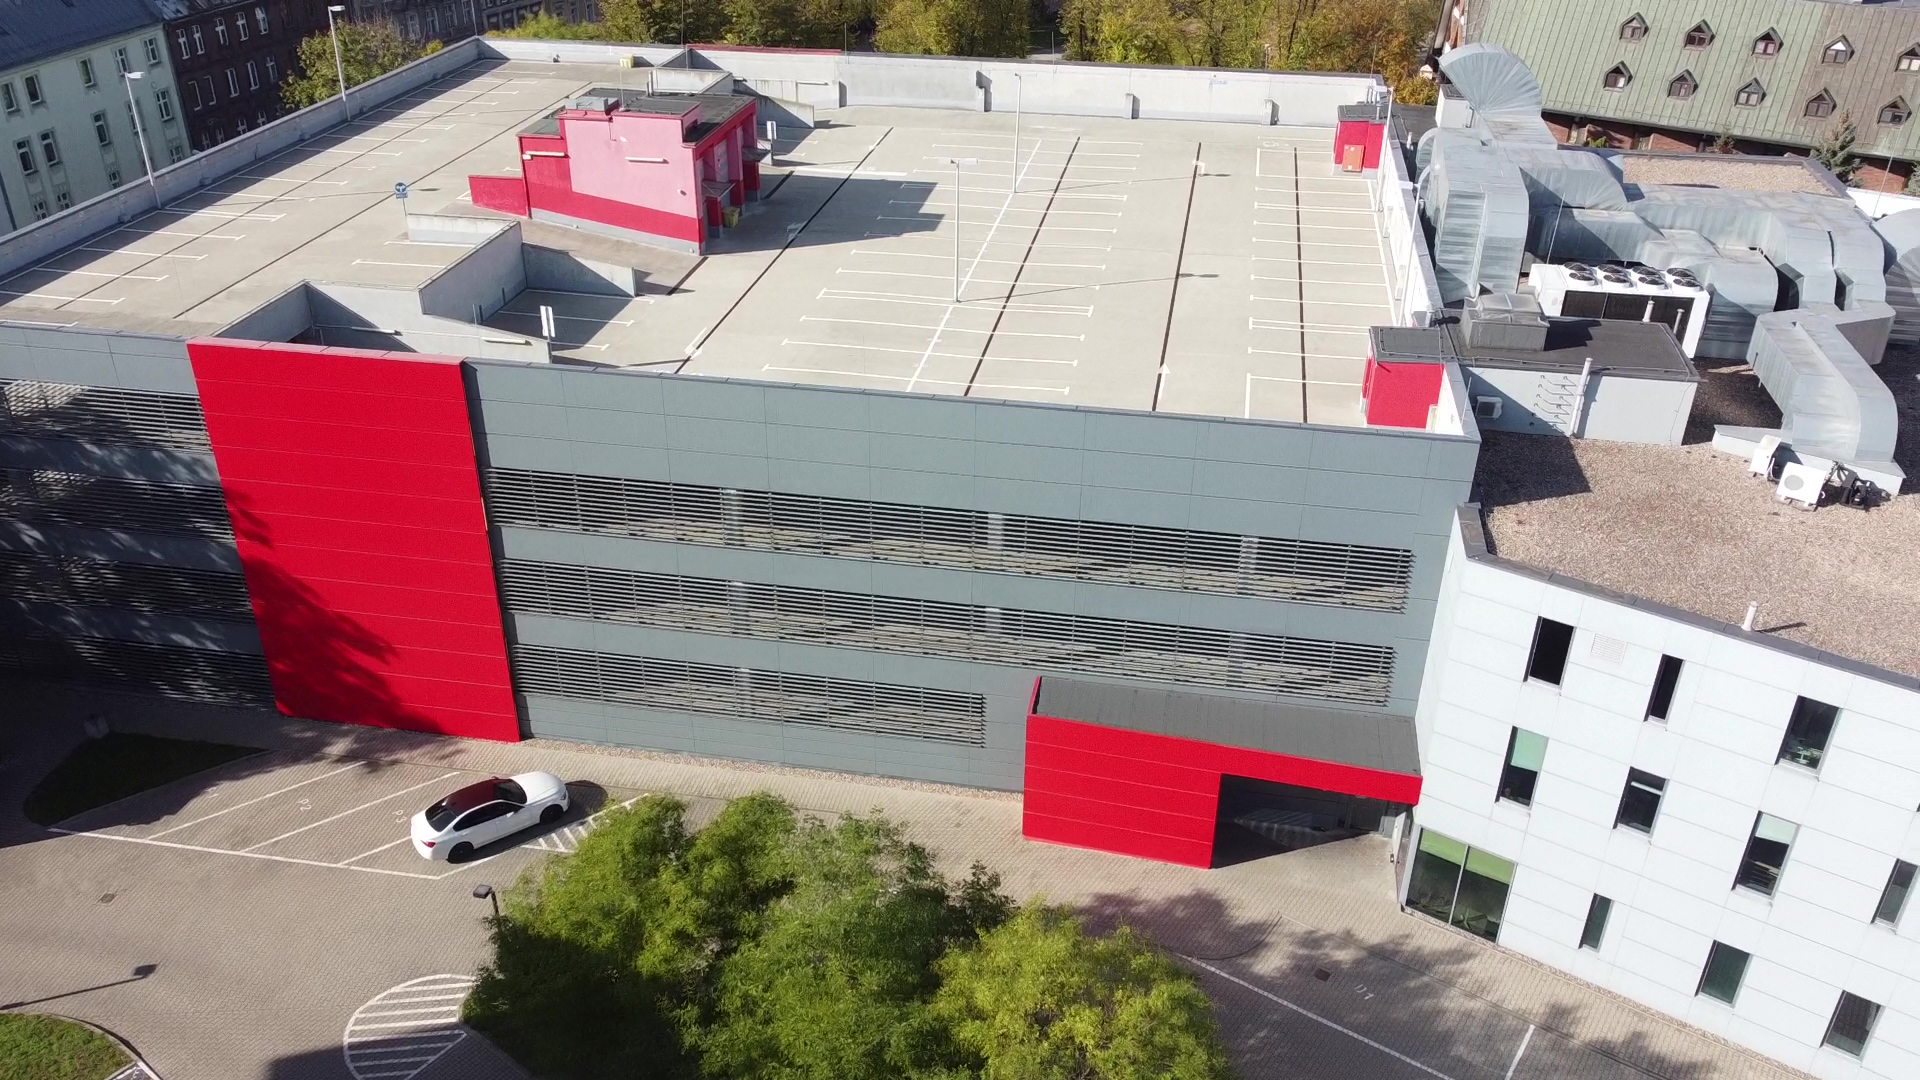
\includegraphics[width=\textwidth]{images/sks_dataset_1.jpg}
    \end{minipage}
    \hfill
    \begin{minipage}{0.245\textwidth}
        \centering
        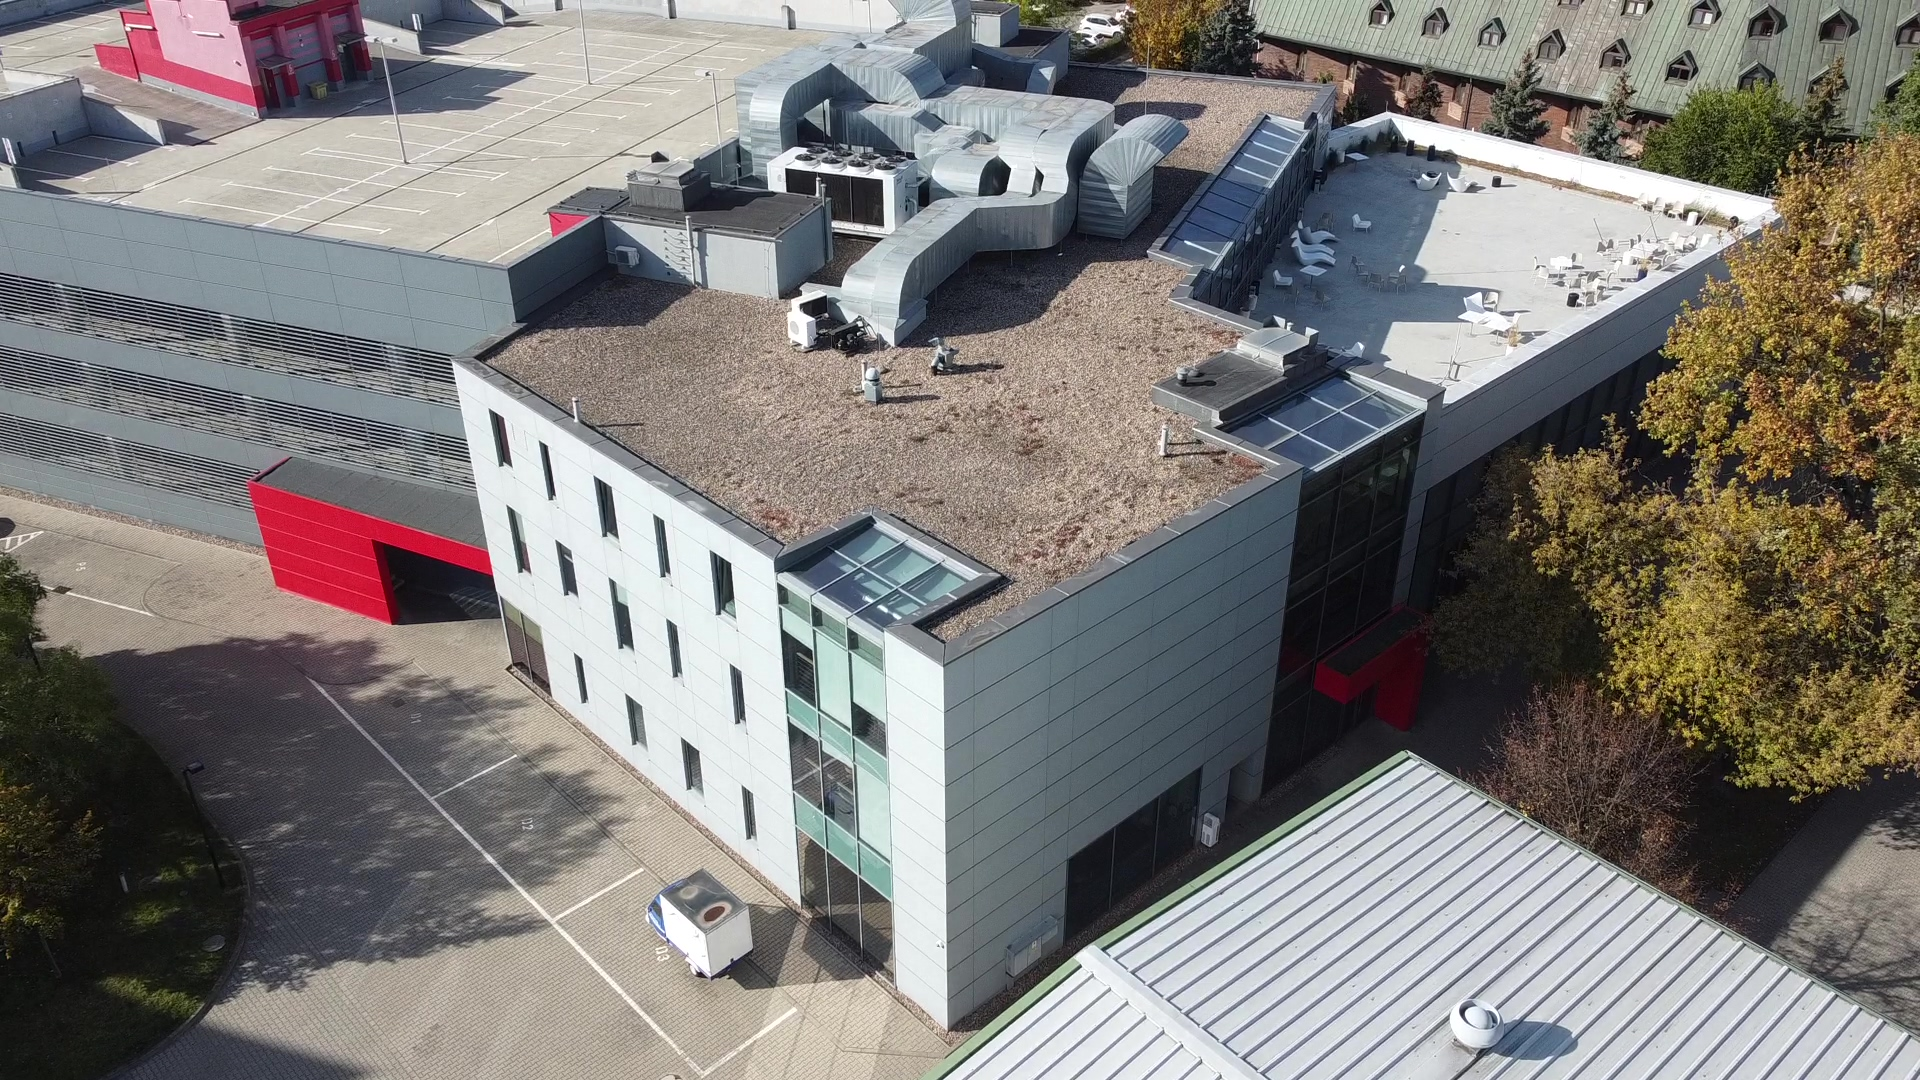
\includegraphics[width=\textwidth]{images/sks_dataset_2.jpg}
    \end{minipage}
    \hfill
    \begin{minipage}{0.245\textwidth}
        \centering
        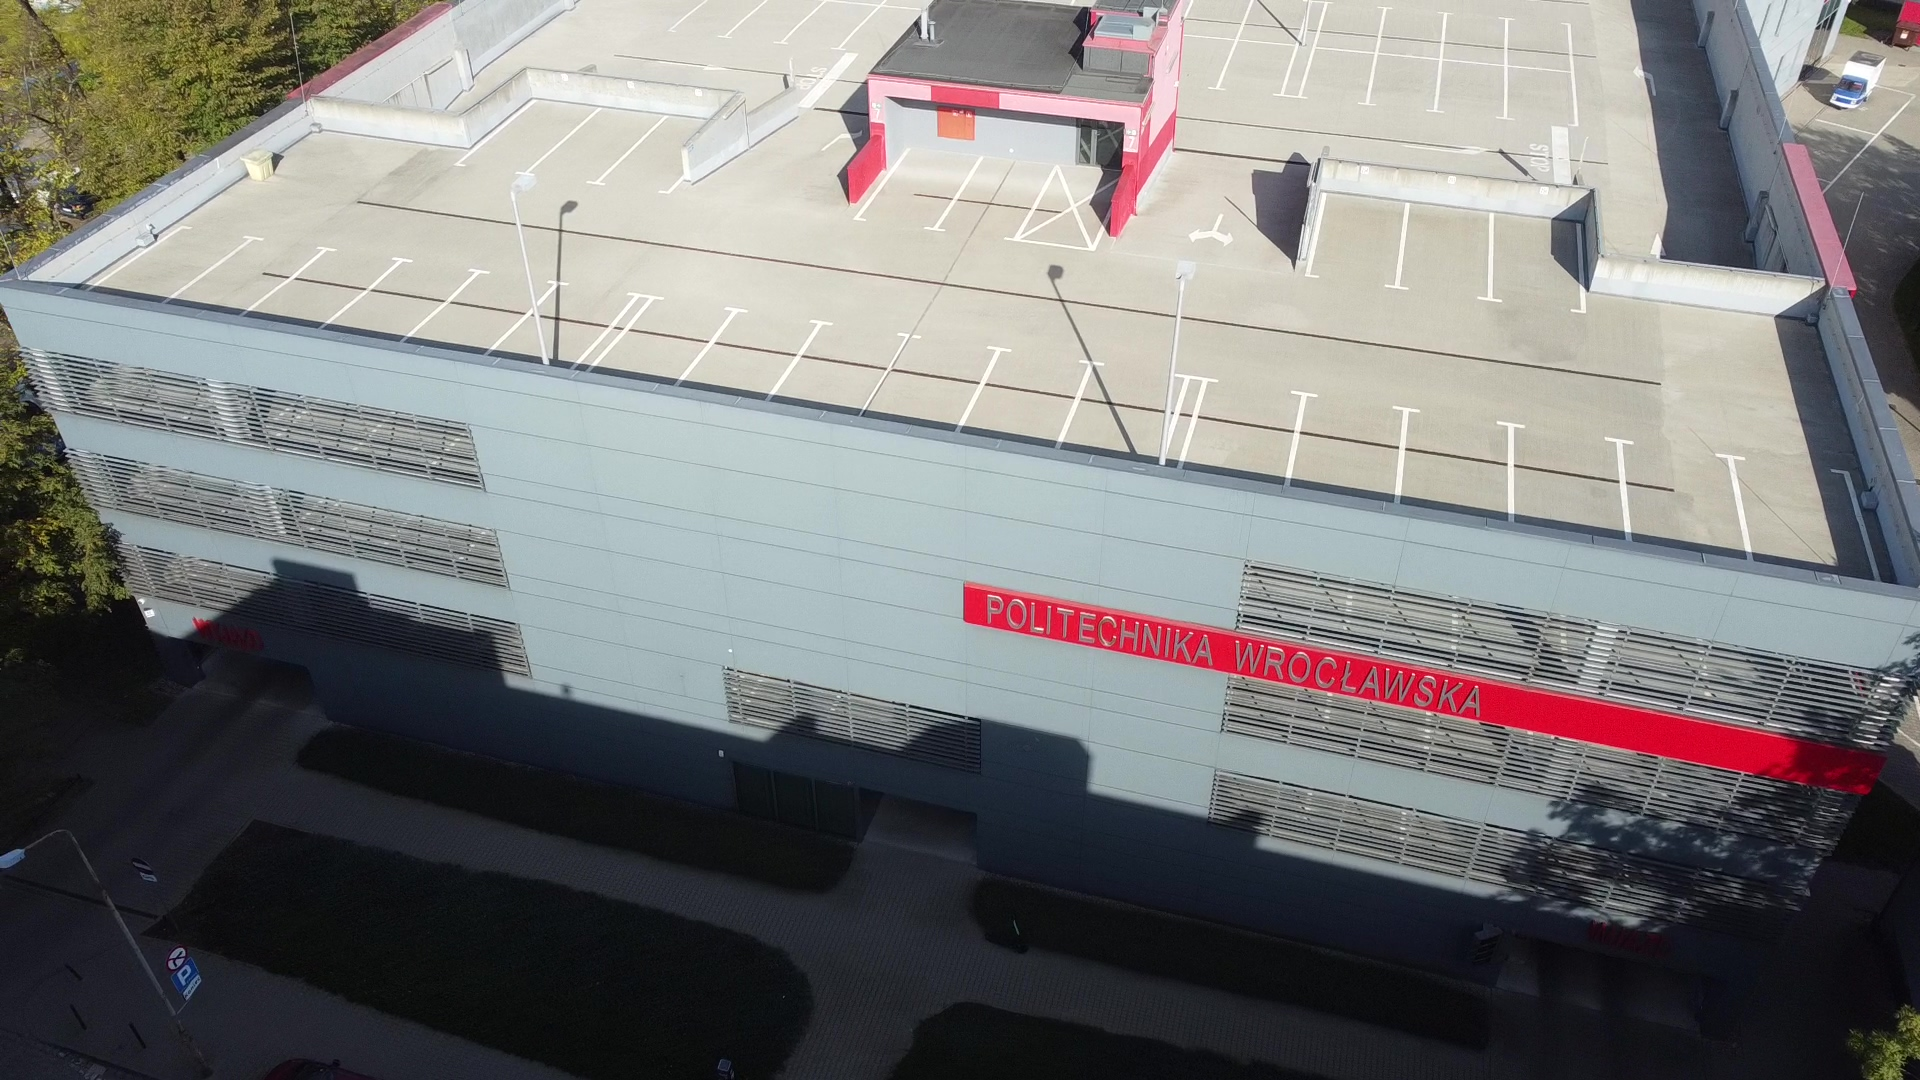
\includegraphics[width=\textwidth]{images/sks_dataset_3.jpg}
    \end{minipage}
    \hfill
    \begin{minipage}{0.245\textwidth}
        \centering
        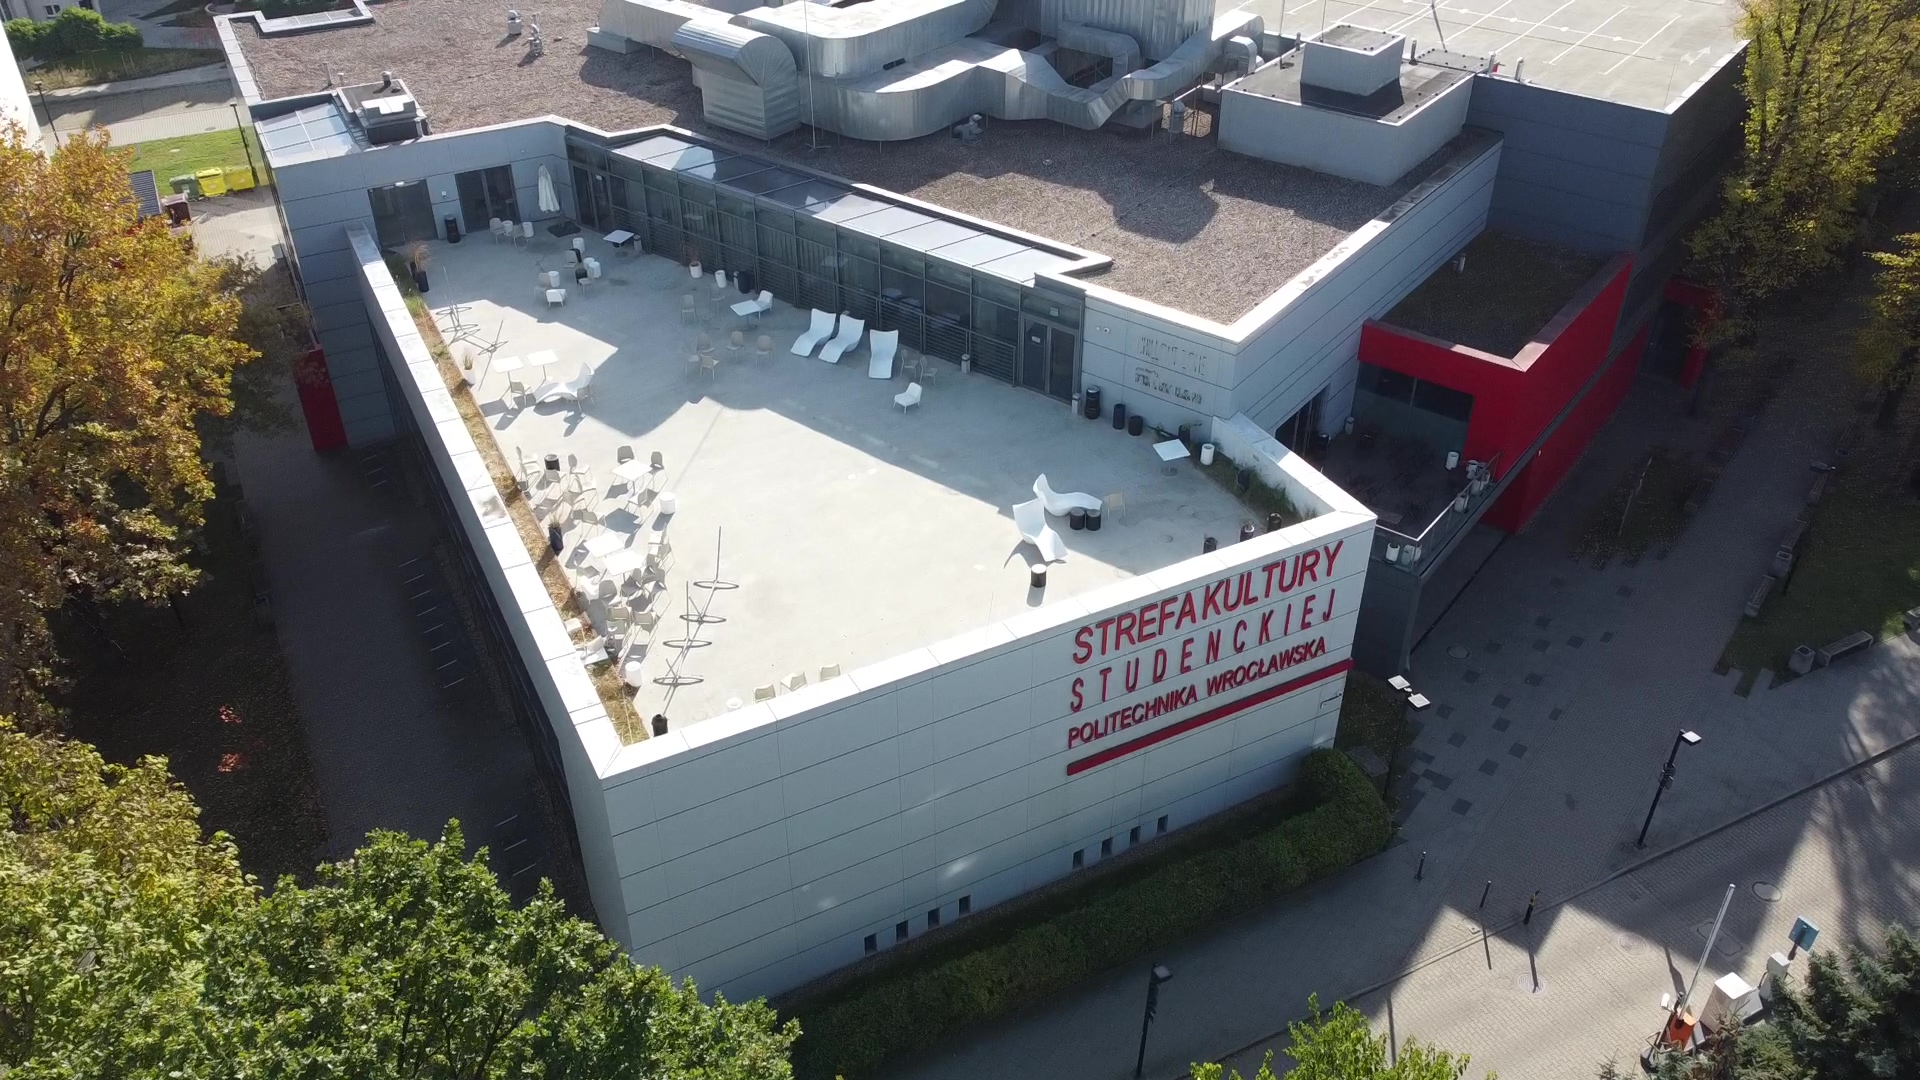
\includegraphics[width=\textwidth]{images/sks_dataset_4.jpg}
    \end{minipage}
    \caption{Przykładowe zdjęcia z akwizycji danych przedstawiające SKS}
    \label{fig:four-photos}
\end{figure}

\subsection{Structure from motion}
Kolejnym etapem projektu było wykorzystanie techniki \textit{Structure from Motion} (SfM) do wyznaczania
struktur przestrzennych scen na podstawie dobranych zestawów zdjęć dwuwymiarowych. 

Algorytmy SfM, identyfikując i łącząc 
punkty wspólne między zdjęciami, ustalają zarówno rozmieszczenie tych punktów w przestrzeni, jak i pozycje 
i orientacje kamer, z których wykonano zdjęcia. Proces ten pozwala na oszacowanie struktury trójwymiarowej
sfotografowanego obszaru, czyli wygenerowanie chmury punktów odwzorowującej scenę w postaci 
zbioru punktów 3D o przypisanych kolorach, tak jak to pokazano na \ref{fig:example_recon}. 

Do realizacji tego zadania użyliśmy popularnego narzędzia COLMAP, a konkretnie jego wersji w formie biblioteki 
\textit{pycolmap}, oferującej funkcjonalności m.in. do wykrywania charakterystycznych cech na obrazach, 
łączenia punktów wspólnych na zdjęciach czy przeprowadzania rekonstrukcji sceny 3D na podstawie dopasowań 
między nimi.

Uzyskana w ten sposób trójwymiarowa reprezentacja sceny w postaci chmury punktów służy za podstawę do 
modelowania z zastosowaniem algorytmu Gaussian Splatting. 

\begin{figure}[!ht]
    \centering
    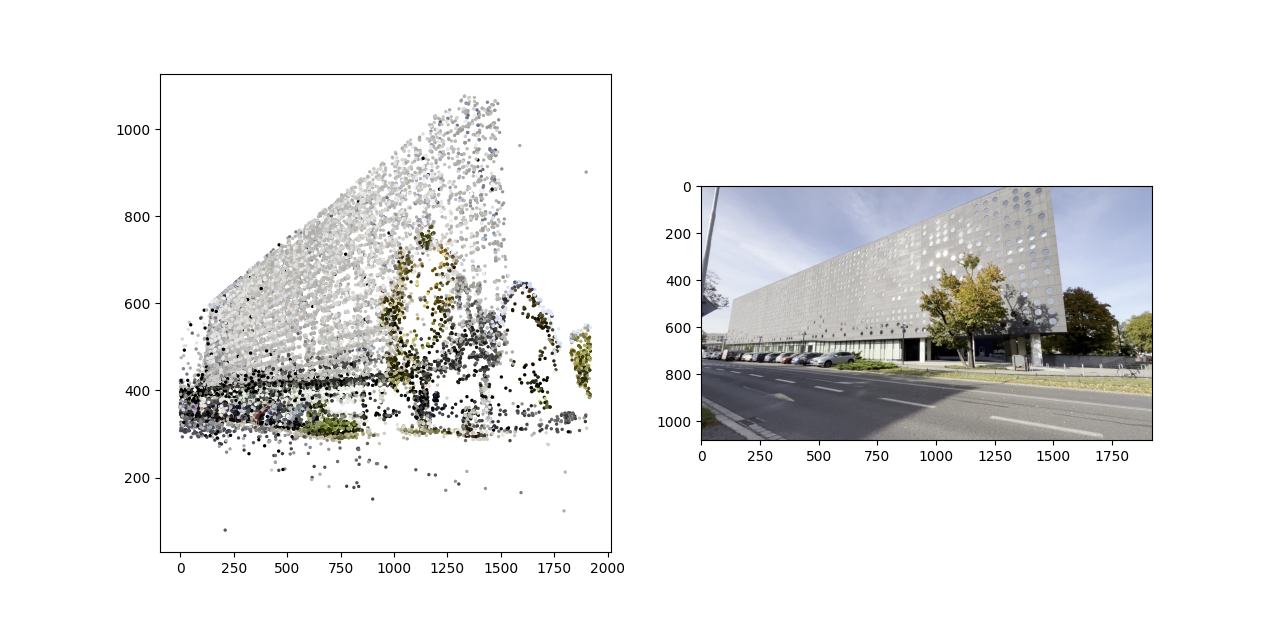
\includegraphics[width=0.9\linewidth]{images/sfm.png}
    \caption{Projekcja przykładowej chmury punktów na płaszczyznę porównana do zdjęcia}
    \label{fig:example_recon}
\end{figure}

\subsection{Gaussian Splatting}
Przy pomocy biblioteki \textit{gsplat}\cite{ye2024gsplatopensourcelibrarygaussian} zawierającej implementację \textit{Gaussian Splatting} w Pythonie wykonaliśmy eksperymenty polegające na uruchomeniu algorytmu dla różnych wartości hiperparametrów w celu znalezienia wartości, które prowadzą do jak najbardziej optymalnego procesu trenowania w kontekście czasu trwania i wykorzystania pamięci. 

Na wejściu algorytmu podawana jest otrzymywana w procesie rekonstrukcji chmura punktów, która jest bazą do dalszego dzielenia i powstawania "gaussianów", a ich parametry: pozycja, kolor, skala i rotacja są optymalizowane przy pomocy metody spadku wzdłuż gradientu. Metryki przyjęte do oceny jakości to SSIM (Structural Similarity Index Measure), PSNR (Peak Signal-to-Noise Ratio) oraz LPIPS (Learned Perceptual Image Patch Similarity).

W wyniku przeprowadzenia eksperymentów okazało się, że najważniejszymi sterującymi procesem parametrami są 
\begin{enumerate}
    \item Liczba Gaussianów: w przypadku scen urbanistycznych w celu oddania odpowieniej szczegółowości potrzebne jest parę milionów Gaussianów, dla naszych scen było to zwykle 3 mln.
    \item Strategia i częstość adaptacji: określają w jaki sposób oraz jak często dodawane i usuwane są Gaussiany. 
    \item Liczba iteracji: zwykle im dłużej trenowana jest scena tym lepsze wyniki otrzymujemy, jednak zależy to również od przyjętej strategii. Liczba ta wpływa bezpośrednio na czas trenowania, powinna wynieść nie mniej niż paręnaście tysięcy.
    \item Stopień zmiennych harmonicznych: wyrażają one kolor, im większy stopień tym lepsza jakość sceny, ale też zwiększone zużycie pamięci i wydłużony czas trenowania. 
\end{enumerate}

Poniżej przedstawione są przykładowe wizualizacje. Renderowania zostały wykonane przy pomocy biblioteki nerfview która również służy do wizualizacji splatów. Na poniższych rysunkach są od lewej do prawej: prawdziwe zdjęcie i widok modelu.

\begin{figure}[!h]
    \centering
    \includegraphics[width=1.0\linewidth]{images/sks_viper_0008.png}
    \caption{Scena SKS}
    \label{fig:sks_gs}
\end{figure}

\begin{figure}[!h]
    \centering
    \includegraphics[width=1.0\linewidth]{images/c5_mouse_0001.png}
    \caption{Scena C5}
    \label{fig:c5_gs}
\end{figure}

\begin{figure}[!h]
    \centering
    \includegraphics[width=1.0\linewidth]{images/c7_gepard_0006.png}
    \caption{Scena C7}
    \label{fig:c7_gs}
\end{figure}

\begin{table}[!h]
    \centering
    \begin{tabular}{|c|c|c|c|c|}
    \hline
    scena & PSNR & SSIM & LPIPS & liczba gaussianów \\
    \hline 
    SKS & 22.03 & 0.71 & 0.25 & 2,937,549 \\
    \hline 
    C5 & 0.0 & 0.0 & 0.0 & 0.0 \\
    \hline 
    C7 & 22.63 & 0.72 & 0.29 & 3,000,000 \\
    \hline
    \end{tabular}
\caption{Całościowe metryki dla testowych scen}
\label{table:tab_conf_sks}
\end{table}

\subsection{Segmentacja semantyczna}
Otrzymana w wyniku poprzednich etapów chmura punktów poddawana procesowi segmentacji semantycznej, czyli przypisaniu każdemu z punktów odpowiedniej kategorii semantycznej opisującej obiekt, w skład którego wchodzi. Do wybranych (na podstawie popularnych w literaturze zbiorów danych służących za punkt odniesienia w testowaniu modeli) kategorii semantycznych należą między innymi \textit{budynek}, \textit{droga}, czy też \textit{zieleń miejska}. 
Używając biblioteki \textit{PyTorch} do uczenia głębokiego, w oparciu o istniejące rozwiązania i aktualny stan wiedzy, przygotowano i wytrenowano własne modele \emph{sieci neuronowych} do segmentacji semantycznej.
W procesie eksperymentowania z różnymi architekturami i sposobami implementacji procesu treningu i predykcji za kluczowe pod względem wpływu na osiągi otrzymanego modelu należy uznać:
\begin{enumerate}
    \item próbkowanie - przy przetwarzaniu zbiorów danych, w przypadku których określenie porządku jest z punktu widzenia efektywności rozwiązania bezcelowe, a które jednocześnie z punktu widzenia modelu mogą osiągać różne rozmiary, ważnym elementem procesu zarówno treningu, jak i predykcji jest odpowiednie próbkowanie całego zbioru. Jest to niezbędne ze względu na architekturę sieci neuronowych, która zakłada stały rozmiar wejścia do modelu. W obrębie tego problemu należy wyróżnić następujące czynniki:
    \begin{enumerate}
        \item rozmiar próbki - zbyt mały może uniemożliwić uchwycenie zależności pomiędzy zbliżonymi do siebie w chmurze punktami,
        \item sposób próbkowania - wpływa na zależność uchwyconych w wyniku procesu uczenia wzorców od bardziej lub mniej odległych od siebie punktów. Może prowadzić do swego rodzaju zdominowania segmentowanych punktów przez jedną kategorię.
    \end{enumerate}
    \item niezbalansowany zbiór danych - w przypadku rozpatrywania dużych scen miejskich naturalnym jest pojawienie się mniej (\textit{samochody}, \textit{tory kolejowe}) i bardziej (\textit{budynki}) popularnych kategorii semantycznych. Jest to klasyczny problem uczenia maszynowego na niezbalansowanym zbiorze danych, który, niezaadresowany, prowadzi do dominacji zbioru przez punkty popularniejszych kategorii, w efekcie przekładając się na słabszą generalizację otrzymanego modelu, w szczególności dla mniej popularnych kategorii semantycznych. W toku prac rozważano dwa sposoby radzenia sobie z tym problemem:
    \begin{enumerate}
        \item próbkowanie - opisane wyżej,
        \item ważenie funkcji straty - \textit{karze} model za omijanie mniej popularnych kategorii semantycznych. Technika ta może prowadzić do nadreprezentacji tych kategorii w otrzymanym w wyniku predykcji zbiorze, jednakże przy odpowiedniej implementacji nieco słabsze wartości metryk dla popularnych kategorii są \textit{nomen omen} balansowane przez lepsze wyniki na niedoreprezentowanych w zbiorze treningowym kategorii, prowadząc w efekcie do lepszych wartości metryk dla całego zbioru testowego.
    \end{enumerate}
    \item dobór danych treningowych, walidacyjnych i testowych - typowy problem dla uczenia maszynowego. Dbając o generalizację modelu nie możemy dopuścić do \textit{wycieku danych}, tj. sytuacji, w której obiecujące wyniki są spowodowane nie ową generalizacją, a pewnego rodzaju pokrewieństwem danych służących do treningu modelu i jego oceny w trakcie tego procesu lub po jego zakończeniu. Rozwązaniem oprócz odpowiedniego podziału i doboru danych jest użycie technik przetwarzania chmur punktów związanych np. z ich obracaniem lub skalowaniem, tak aby wyuczone wzorce podlegały jak najlepszemu uogólnieniu.
\end{enumerate}

\begin{table}[!h]
    \centering
    \begin{tabular}{|c|c|c|c|c|c|c|}
    \hline
    scena & PSNR & SSIM & LPIPS & liczba gaussianów & czas trenowania & pamięć pliku (MB) \\
    \hline 
    SKS & 22.03 & 0.71 & 0.25 & 2,937,549 & 2h53m & 661 \\
    \hline 
    C5 & 21.98 & 0.71 & 0.26 & 4,564,464 & 10h40m & 675 \\
    \hline 
    C7 & 22.63 & 0.72 & 0.29 & 3,000,000 & 15h15m & 675 \\
    \hline
    \end{tabular}
\caption{Całościowe metryki dla testowych scen. Otrzymane wartości PSNR, SSIM oraz LPIPS zwykle świadczą o dobrej jakości scenie, która oddaje wystarczające szczegóły i wygładzone artefakty.}
\label{table:tab_seg_met}
\end{table}

Otrzymany w wyniku tego procesu eksperymentowania model wdrożono w celu jego używania na \textit{niewidzianych} przez niego dotychczas danych.

\subsection{Wizualizacja}
W celu zapewnienia użytkownikowi końcowemu zintegrowanego i spójnego środowiska wizualizacji całego procesu – od wgrania plików wejściowych po interakcję z modelem – zaprojektowano od podstaw interfejs oraz system renderowania.

Założeniem projektu była implementacja intuicyjnego, dynamicznego i responsywnego \textbf{interfejsu}[\ref{fig:ui}] przy pomocy biblioteki \textit{PyQt} oraz języka \textit{QML}. Interfejs został zintegrowany z wydajnym systemem \textbf{renderingu}[\ref{fig:rendering}] GPU, wykorzystującym technologie \textit{OpenGL}, \textit{OpenCL} oraz język \textit{C}. Dodatkowo, użytkownik ma możliwość alternatywnego renderowania z wykorzystaniem biblioteki \textit{VisPy}.

Projekt rozwiązuje problem fragmentaryczności funkcji dostępnych w innych aplikacjach, oferując spójne środowisko do obsługi modeli 3D, obejmujące procesy tworzenia, modyfikacji, segmentacji oraz wizualizacji danych.
\\[10pt]
\textbf{Funkcjonalności interfejsu}

\begin{itemize} \item wybór zdjęć, \item ustawienie parametrów, \item generowanie chmury punktów, \item generowanie splatów, \item segmentacja splatów, \item wizualizacja wyników. \end{itemize}

\vspace{10pt}
{\setlength{\parindent}{0pt}
\textbf{Rendering}
}

Rendering wykorzystuje plik .ply jako dane wejściowe do wczytania splatów. Splaty te są reprezentowane przez sześciany z dodatkowymi parametrami przechowywanymi w Shader Storage Buffer Object (SSBO), co umożliwia efektywny odczyt dużych ilości danych. Takie podejście jest szczególnie przydatne w przypadku scen zawierających nawet do dwóch milionów obiektów.

Do przechowywanych parametrów należą: \begin{itemize} \item pozycja, \item skala, \item rotacja, \item kolor, \item przezroczystość. \end{itemize}

Podczas procesu renderowania, model sześcianu jest odpowiednio przekształcany na podstawie tych parametrów, co pozwala na uzyskanie splatów na wyjściu. Takie podejście umożliwia abstrakcyjne definiowanie splatów przy jednoczesnym zachowaniu wysokiej dokładności wizualnej.

\clearpage

\begin{figure}[!ht]
    \centering
    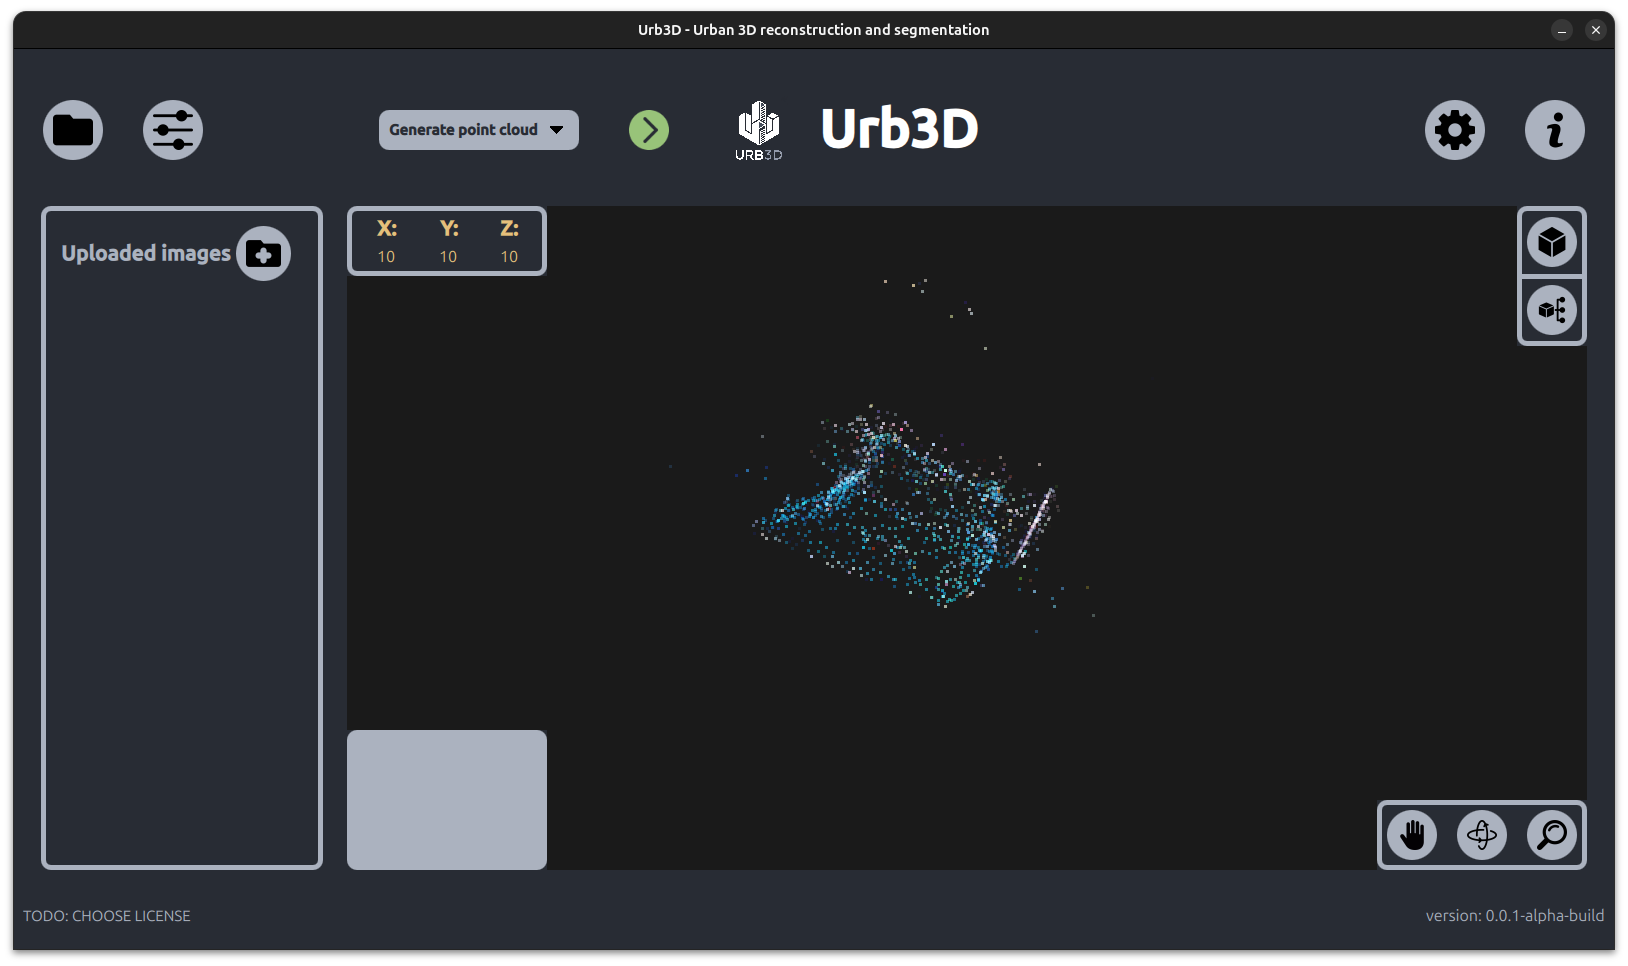
\includegraphics[width=\textwidth]{images/UI-Rendering.png}
    \caption{Zrzut ekranu przedstawiający główny widok aplikacji}
    \label{fig:ui}
\end{figure}

\begin{figure}[!ht]
    \centering
    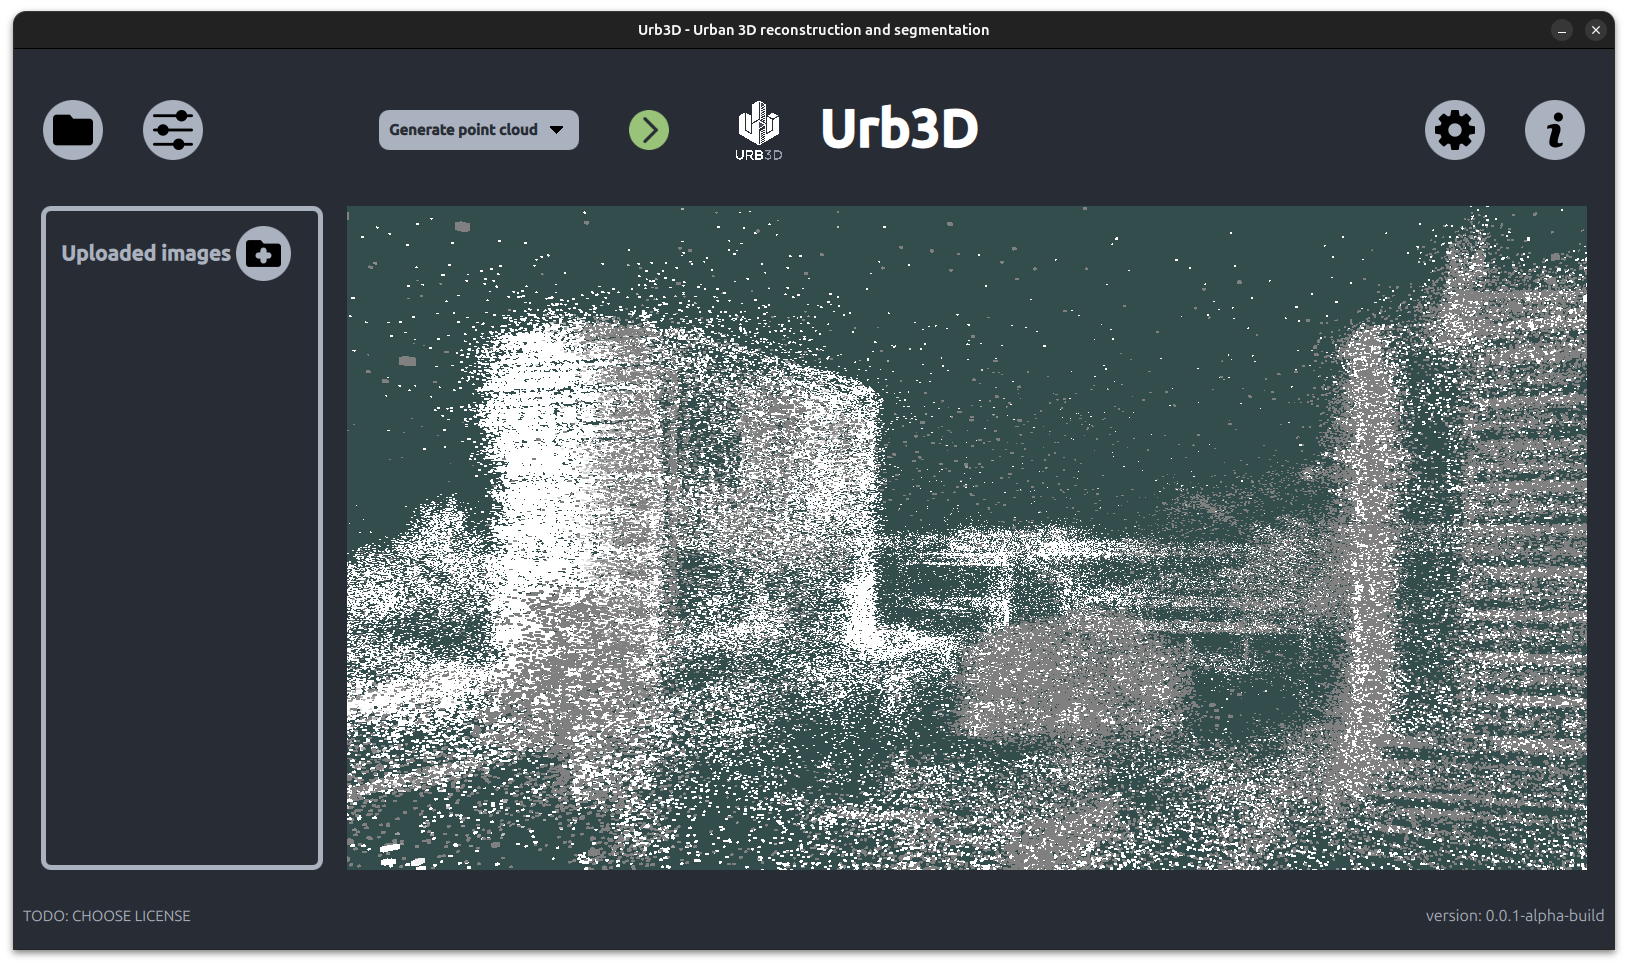
\includegraphics[width=\textwidth]{images/cloud_rendering.png}
    \caption{Zrzut ekranu przedstawiający własny renderer}
    \label{fig:rendering}
\end{figure}

\section{Podsumowanie}
\subsection{Osiągnięcie zamierzonych celów}

W ramach oceny projektu rozpatrzono osiągnięcie celów wyznaczonych na początku jego projektowania:

\begin{enumerate}
    \item skomponowanie własnego zbioru danych - przeprowadzono akwizycję danych na podstawie budynków Politechniki Wrocławskiej,
    \item wykorzystanie algorytmu Gaussian Splatting do rekonstrukcji sceny 3D - przystosowano skrypty implementujące algorytm Gaussian Splattingu do problemu dużych scen miejskich,
    \item filtracja chmury punktów przy użyciu różnych technik - w celu polepszenia osiągów modeli przed i po splattingu następują różne filtracje chmury punktów,
    \item zastosowanie architektur sieci neuronowych takich jak PointNet do klasyfikacji chmury punktów - wytrenowano i opisano model PointNet do segmentacji scen miejskich,
    \item adaptacja istniejących bibliotek do wizualizacji wyników - wdrożono alternatywne do własnego renderingu metody wizualizacji efektów Gaussian Splattingu i chmury punktów, bazujące na istniejących bibliotekach, 
    \item implementacja własnego algotymu do renderowania gaussianów - wytworzono oprogramowanie realizujące niskopoziomowy renderer chmury punktów i gaussianów, umożliwiający optymalną obliczeniowo wizualizację wyników obliczeń.
\end{enumerate}

Analiza potwierdza sprostanie założonym celom projektu.

\subsection{Wnioski}

Pozytywna ewaluacja osiągnięcia zamierzonych celów projektu pozwala uznać przedsięwzięcie za udane. Na szczególną uwagę zasługuje nieopisany, choć wynikający pośrednio z treści dokumentacji rozwój intelektualny w postaci poszerzenia, a w zasadzie zdobycia przez członków projektu wiedzy z obszaru pochodzącego z poza programu studiów inżynierskich, który dzięki niniejszemu projektowi był możliwy do osiągnięcia.

\subsection{Podziękowania}

Szczególne podziękowania należą się operatorce drona Paulinie, bez której z pewnością sukces w obszarze akwizycji danych nie byłby możliwy oraz opiekunowi pracy, dr hab. inż. Markowi Krótkiewiczowi, prof. ucz. oraz opiekunom pomocniczym, dr inż. Marcinowi Jodłowcowi, dr inż. Rafałowi Palakowi oraz dr inż. Zbigniewowi Telcowi.


\printbibliography

\end{document}